\documentclass[9pt]{beamer}
\usetheme{Madrid}
\usepackage{mathtools}
\usepackage[T1]{fontenc}
\usepackage[english,french,spanish,italian]{babel}
\usepackage[useregional]{datetime2}
\usepackage{bm}
\usepackage{esvect}
\usepackage{amsmath}
\usepackage{physics}
\usepackage{empheq}
\usepackage[many]{tcolorbox}
\input{pool/NextDefs.tex}

%$\vv{\bm{L}}

\title{Status and prospects of the NEXT experiment}
 
%\subtitle{Report to the LSC Scientific Committee}
 
\author{J.J. G\'omez Cadenas on behalf of the NEXT collaboration}
 
\institute{Donostia International Physics Center (DIPC)} % (optional)
 
\date[March, 19, 2019] % (optional)
%{PHYSIS, SAN SEBASTIAN: 2-6 OCTOBER 2018}
 
%\logo{\includegraphics[height=0.5cm]{dipc.png}
%\includegraphics[height=0.5cm]{IB.png}}


\tcbset{highlight math style={enhanced,
  colframe=red!60!black,colback=yellow!50!white,arc=4pt,boxrule=1pt,
  }}

\newtcbox{\mybox}[1][]{nobeforeafter,math upper,tcbox raise base,
  enhanced,frame hidden,boxrule=0pt,interior style={top color=green!10!white,
  bottom color=green!10!white,middle color=green!50!yellow},
  fuzzy halo=1pt with green,drop large lifted shadow,#1}
  
%------------------------------------------------------------
%The next block of commands puts the table of contents at the 
%beginning of each section and highlights the current section:

\AtBeginSection[]
{
  \begin{frame}
    \frametitle{Table of Contents}
    \tableofcontents[currentsection]
  \end{frame}
}
%------------------------------------------------------------

\begin{document}
\selectlanguage{english}
%The next statement creates the title page.
\frame{\titlepage}

%---------------------------------------------------------
%This block of code is for the table of contents after
%the title page

\begin{frame}
\frametitle{Table of Contents}
\tableofcontents
\end{frame}

%---------------------------------------------------------


\section{Desperately seeking Majorana}
%\begin{frame}
%\frametitle{The Majorana landscape} 
% \begin{center}
%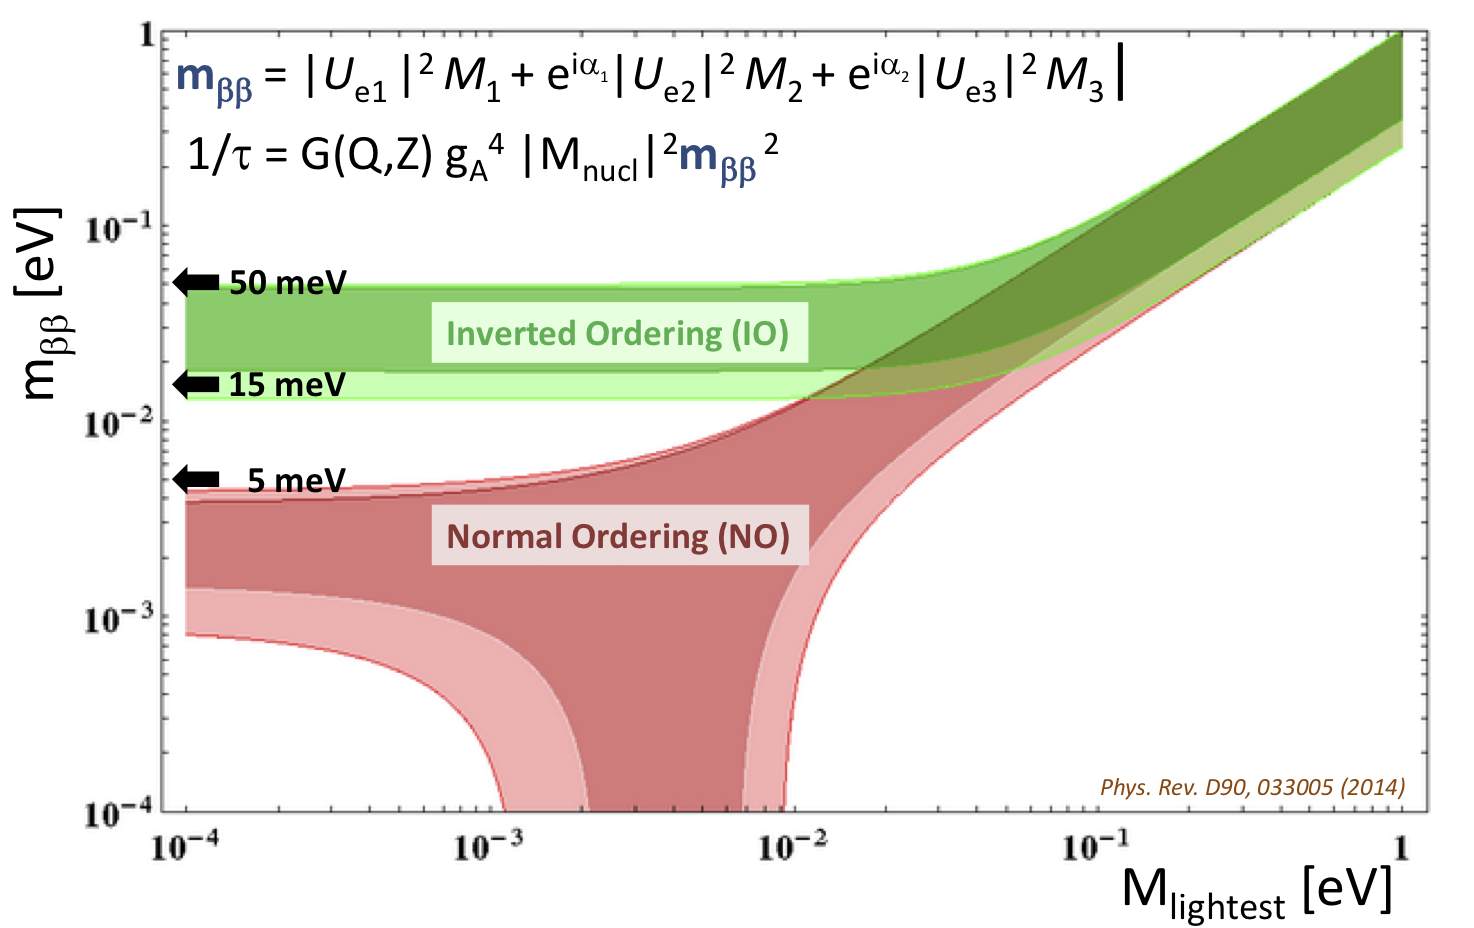
\includegraphics[width=0.75\textwidth]{moriond/landscape.png}
%\end{center}
%\begin{itemize}
%\item {\bf Majorana's  landscape} obtained when plotting \mbb\ vs the lightest neutrino mass.
%\item {\bf Majorana's curse:} Sensitivity to $\mbb \propto to \sqrt{1/\tau}$.
%\end{itemize}
% \begin{flushright}
%{\bf A. Giuliani, Neutrino 2018}
%\end{flushright}
%
%\end{frame}
%
%\begin{frame}
%\frametitle{Connecting \mbb\ with $\tau$} 
% \begin{center}
%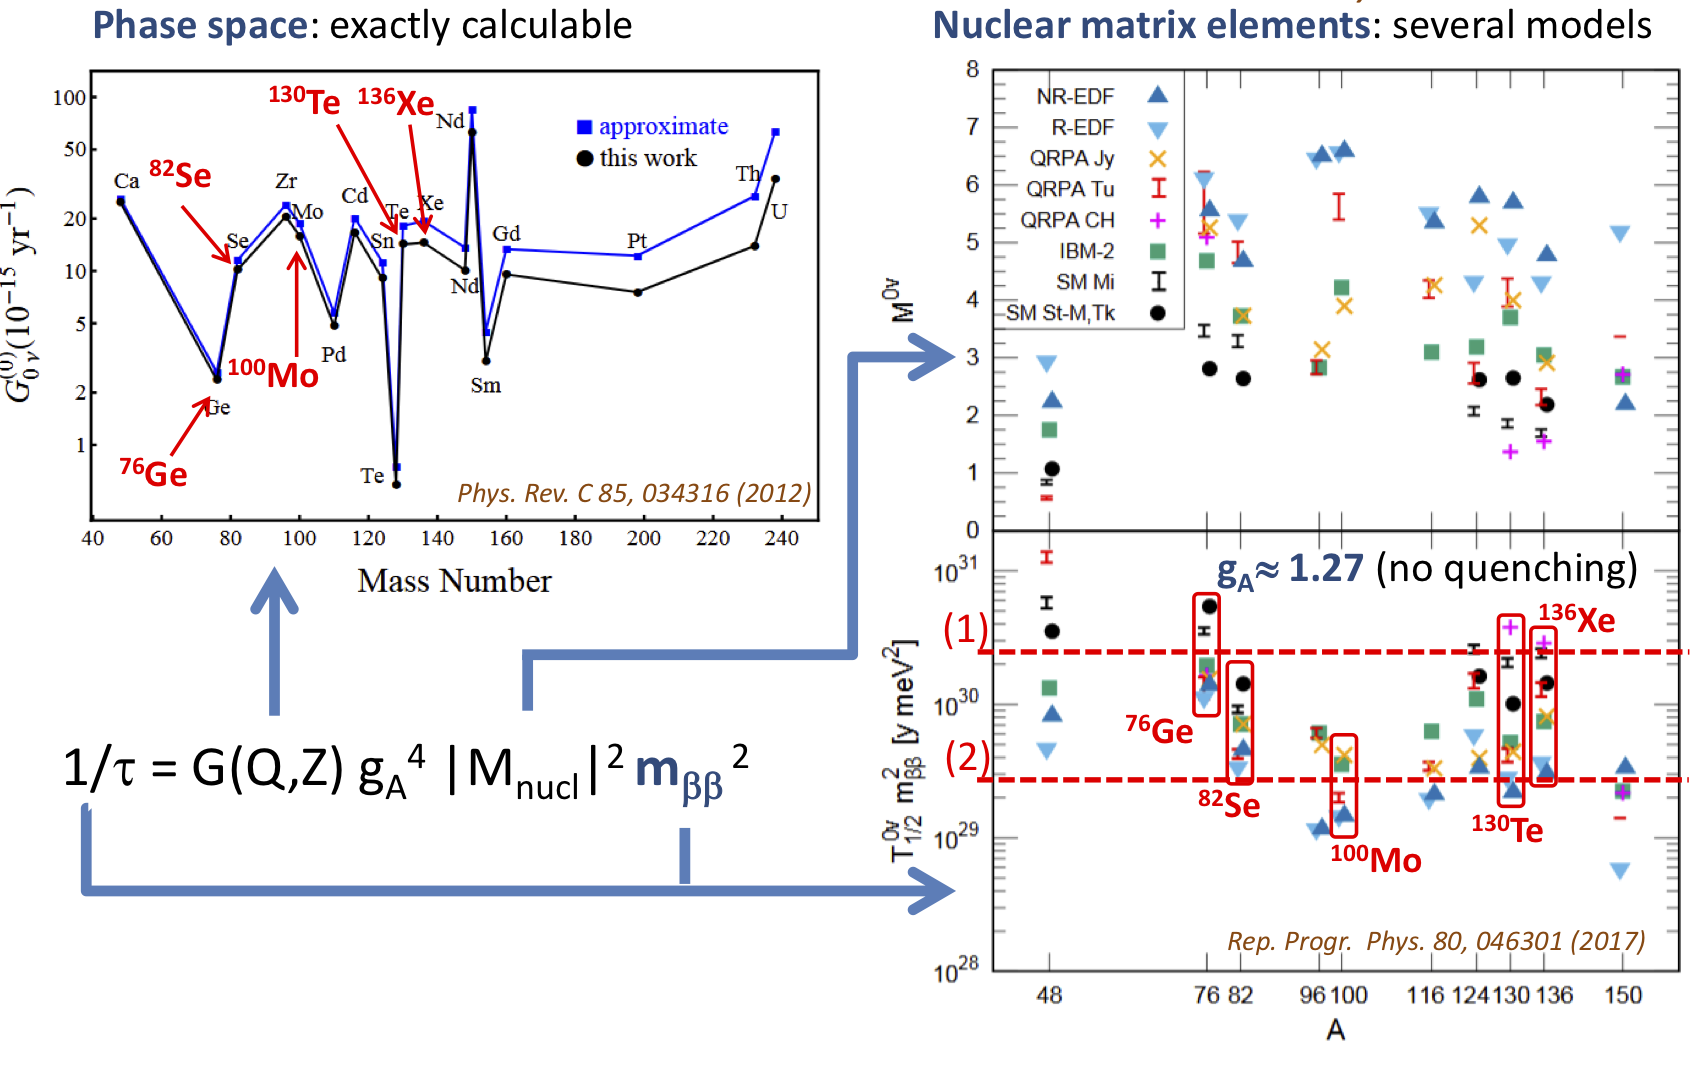
\includegraphics[width=0.75\textwidth]{moriond/nme.png}
%\end{center}
%\begin{itemize}
%\item {\bf case (1):} ``optimistic scenario".
%\item {\bf case (2):} ``pessimistic scenario".
%\end{itemize}
% \begin{flushright}
%{\bf A. Giuliani, Neutrino 2018}
%\end{flushright}
%\end{frame}
%
%\begin{frame}
%\frametitle{Setting the scale} 
% \begin{center}
%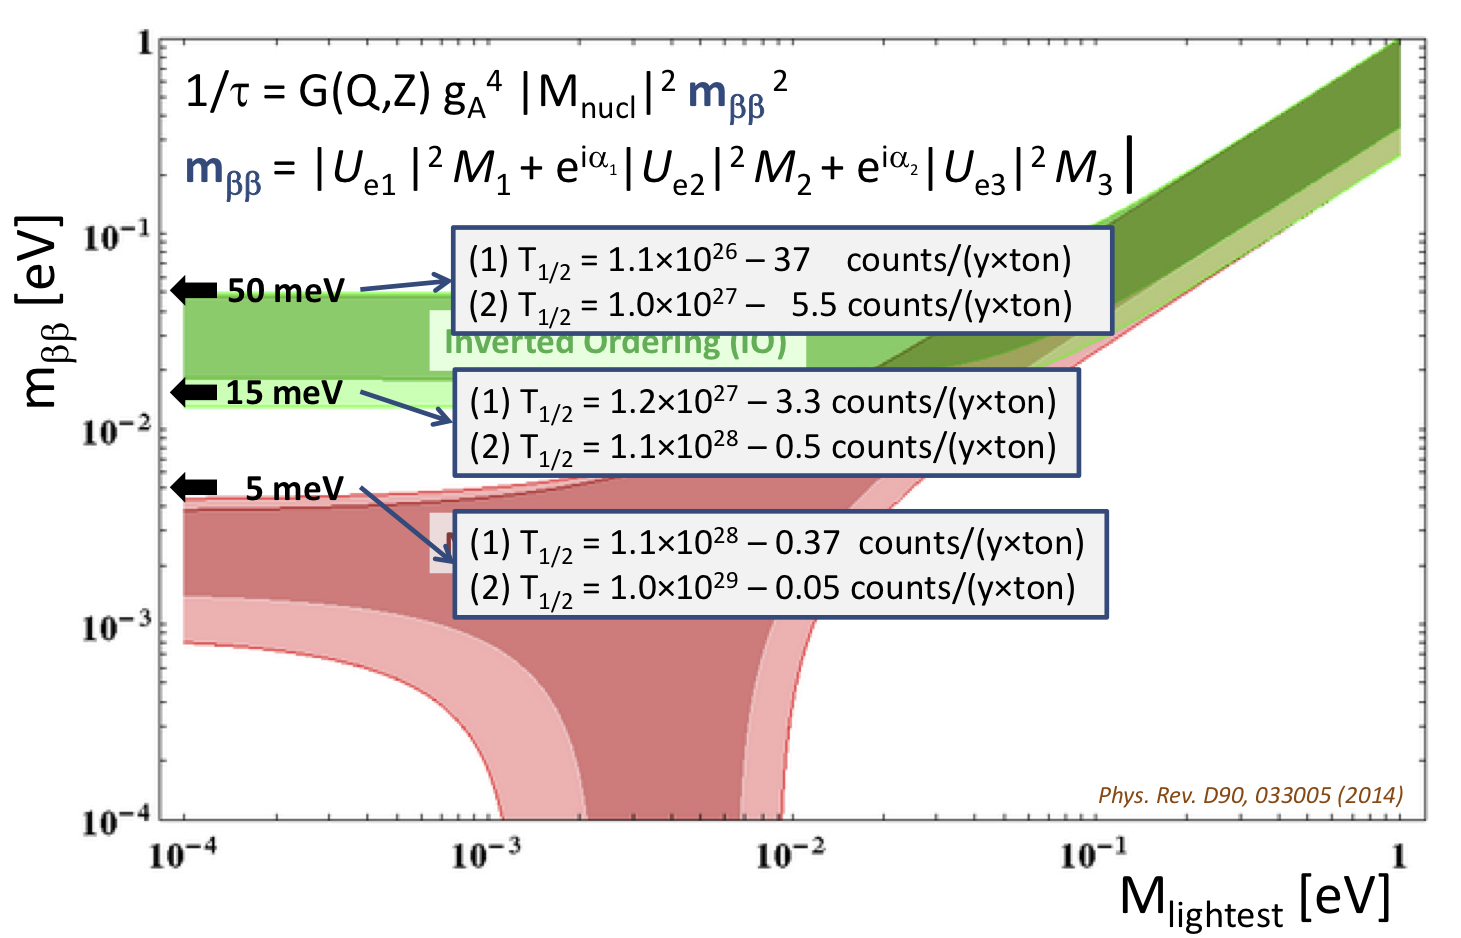
\includegraphics[width=0.75\textwidth]{moriond/setting_the_scale.png}
%\end{center}
%\begin{itemize}
%\item {\bf case (1):}  $\Tonu \sim 10^{27} {\rm yr} \rightarrow \mbb \sim {\rm 15 meV}$, 
%$\Tonu \sim 10^{28} {\rm yr} \rightarrow \mbb \sim {\rm 5 meV}$.
%\item {\bf case (2):} $\Tonu \sim 10^{28} {\rm yr} \rightarrow \mbb \sim {\rm 15 meV}$, 
%$\Tonu \sim 10^{29} {\rm yr} \rightarrow \mbb \sim {\rm 5 meV}$.
%\end{itemize}
% \begin{flushright}
%{\bf A. Giuliani, Neutrino 2018}
%\end{flushright}
%
%\end{frame}

\begin{frame}
\frametitle{Majorana's challenge}

\begin{figure}[tbh!]
  \begin{center}
      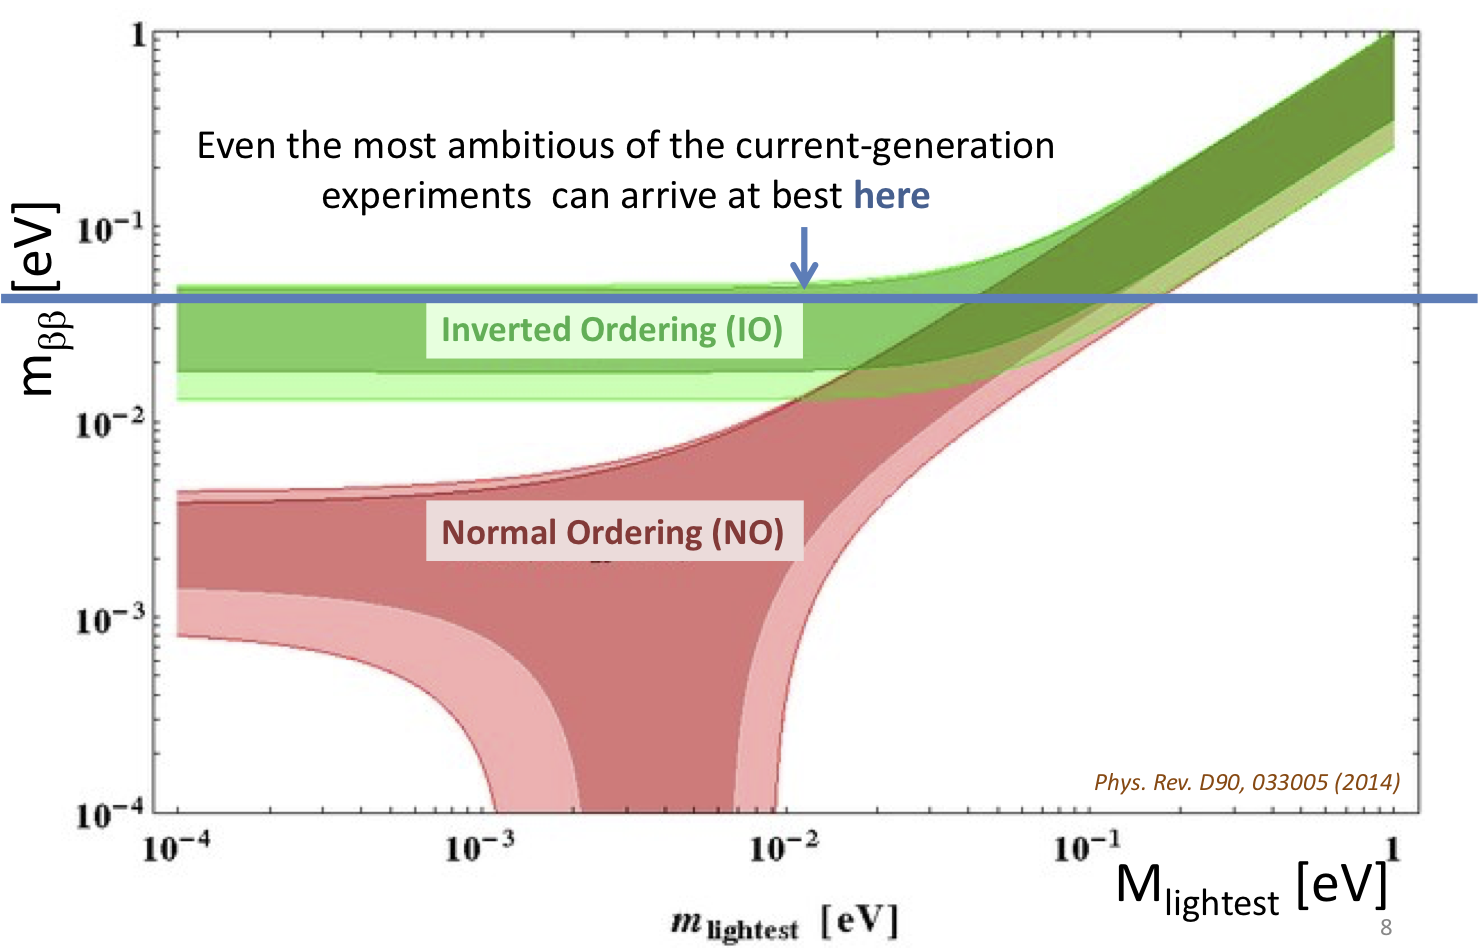
\includegraphics[width=0.45\textwidth]{moriond/current_experiments.png}
       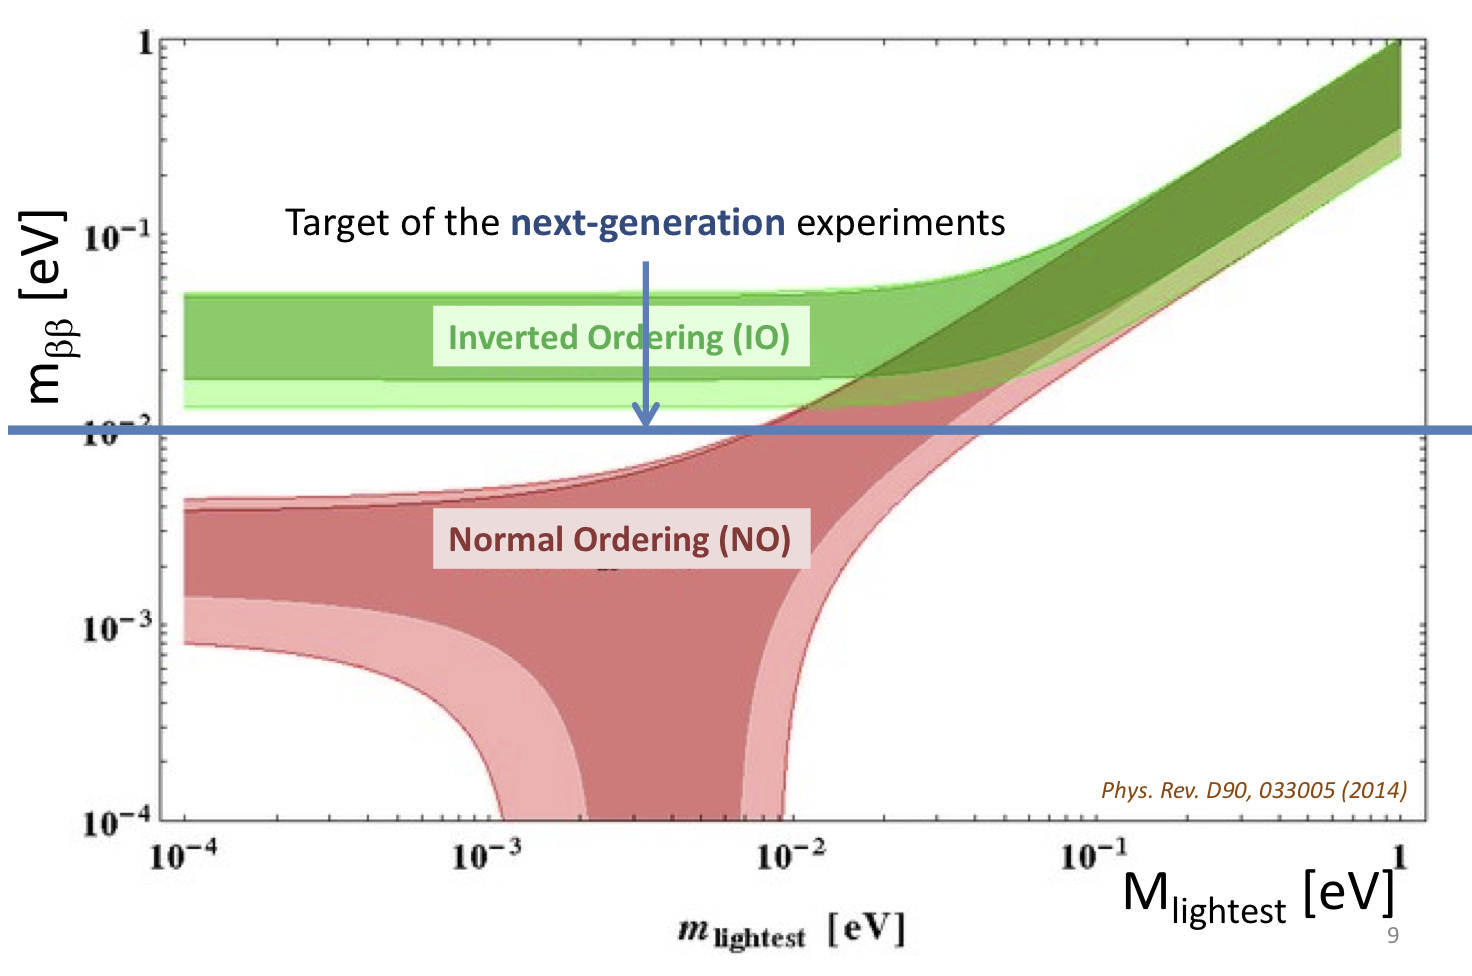
\includegraphics[width=0.45\textwidth]{moriond/nextgen_experiments.png}
      
  \end{center}
\end{figure}
\begin{itemize}
\item {\em Today:} $\Tonu \sim 10^{26} {\rm yr}$.
\item {\em ``Good luck case'':} if $\Tonu \sim 10^{27} {\rm yr}$, observe 3 signal events (per ton and year)  for
$\mbb \sim 15 {\rm ~ meV}$.
\item {\em ``Tough luck case'':} if $\Tonu \sim 10^{28} {\rm yr}$, observe 0.5 signal events (per ton and year) for
$\mbb \sim 15 {\rm ~meV}$.
\item {\bf Bottom line:} {\bf To explore IO exposures in the range of ton (tens of ton) year needed and virtually background free detectors}. 
\end{itemize}
 \begin{flushright}
{\bf A. Giuliani, Neutrino 2018}
\end{flushright}
\end{frame}

%\begin{frame}
%\frametitle{Next generation experiments must be ``background free''}
%
%\begin{columns}
% 
%\column{0.5\textwidth}
%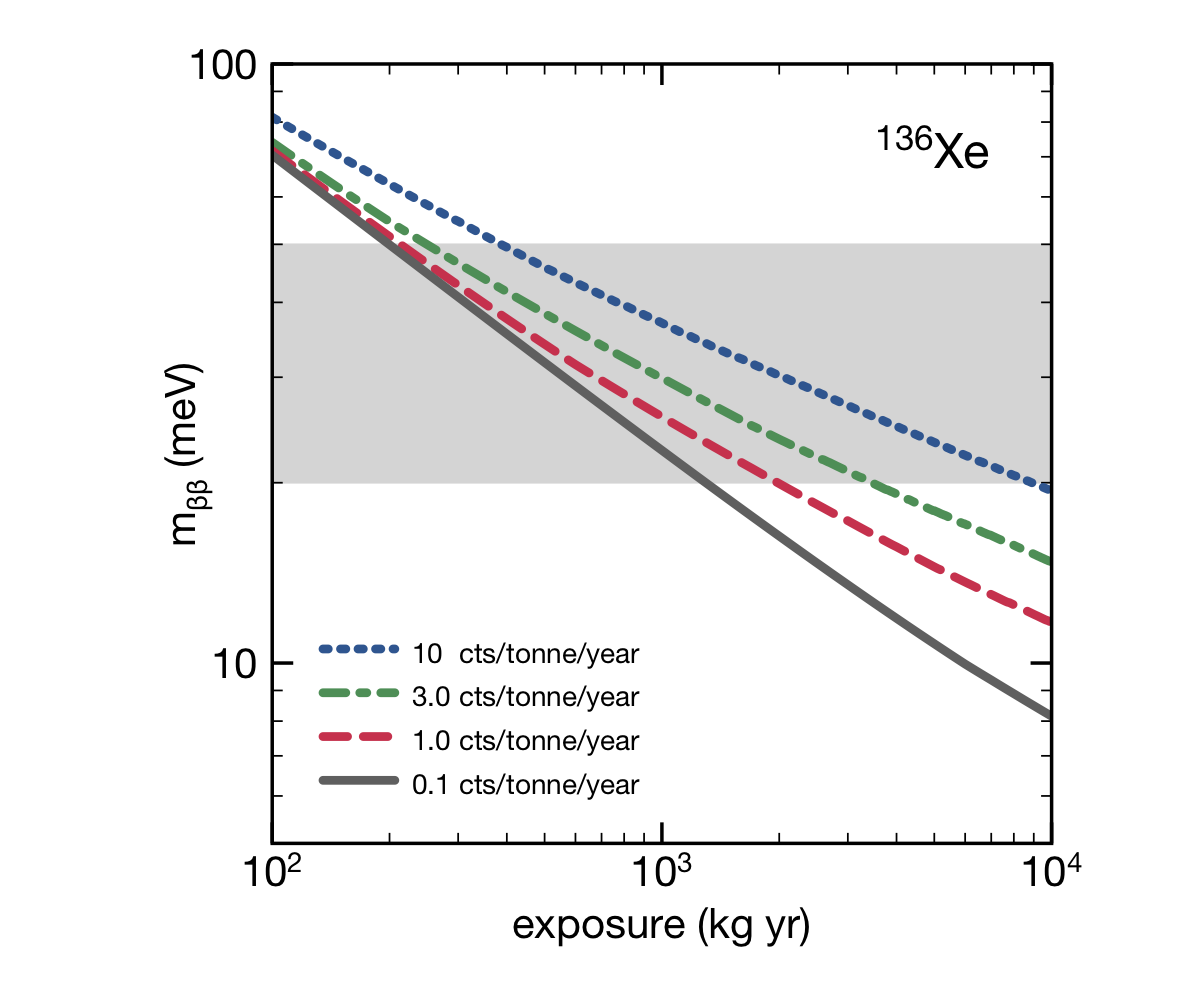
\includegraphics[scale=0.35]{moriond/xenon_bkg.png}
% 
%\column{0.5\textwidth}
%\begin{itemize}
%\item Plot shows the sensitivity of a 100\% efficient Xenon experiment assuming scenario (1).
%\item With a background $\sim$ 10 \ckky\ an exposure of 10 ton years  (30 ton years for an efficiency of 30 \%) is needed to cover the IH.
%\item With a background count of  $\sim$ 1 \ckky\, ``only'' 2 ton years are required (6 ton years for an efficiency of 30\%).
%\item To reach 5 meV in 10 ton years requires a background free (0.1 \ckky) experiment. 
%\end{itemize}
%\end{columns}
%\end{frame}
%
 






\section{Neutrino Experiment with a Xenon TPC (NEXT)}
\begin{frame}
\frametitle{What is NEXT?}

\begin{figure}[tbh!]
  \begin{center}
      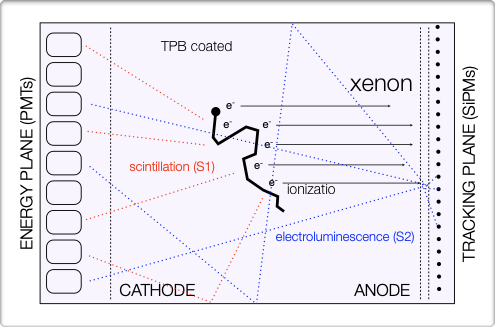
\includegraphics[width=0.45\textwidth]{moriond/next_poo.png}
       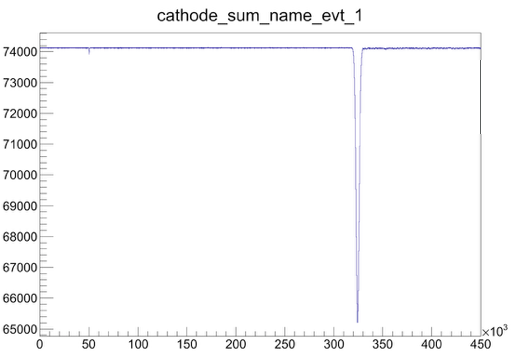
\includegraphics[width=0.45\textwidth]{moriond/next_s1_s2.png}      
  \end{center}
\end{figure}

\begin{itemize}
\item {\bf A HPXe:} High pressure gas chamber (10-20 bar) with EL amplification of the signal. 
\item {\bf Uses xenon,} a noble gas (source$ = $detector) with relatively high \Qbb\ and no long-lived radioactive isotopes. 
\item {\bf An optical TPC:} all signals are light. Primary scintillation (S1) gives \tz\ (needed to fiducialize the event and to correct for finite electron lifetime), EL amplification gives S2, which is used to measure energy and to reconstruct the electron trajectory. 
\end{itemize}
\end{frame}

\begin{frame}
\frametitle{NEXT assets}
\begin{figure}[tbh!]
  \begin{center}
      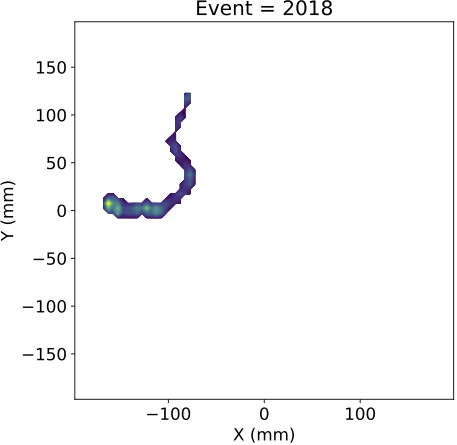
\includegraphics[width=0.20\textwidth]{moriond/single_e.png}
      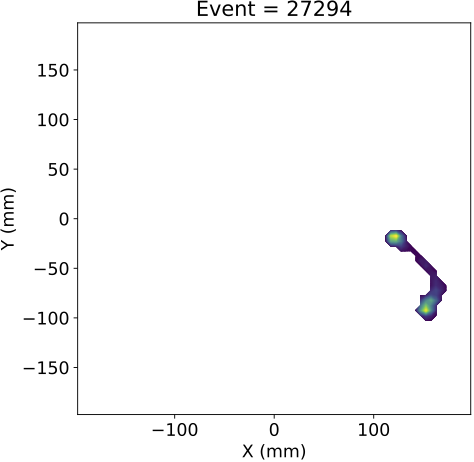
\includegraphics[width=0.20\textwidth]{moriond/double_e.png}
  \end{center}
 \end{figure}
  
 \begin{figure}[tbh!]
  \begin{center}
      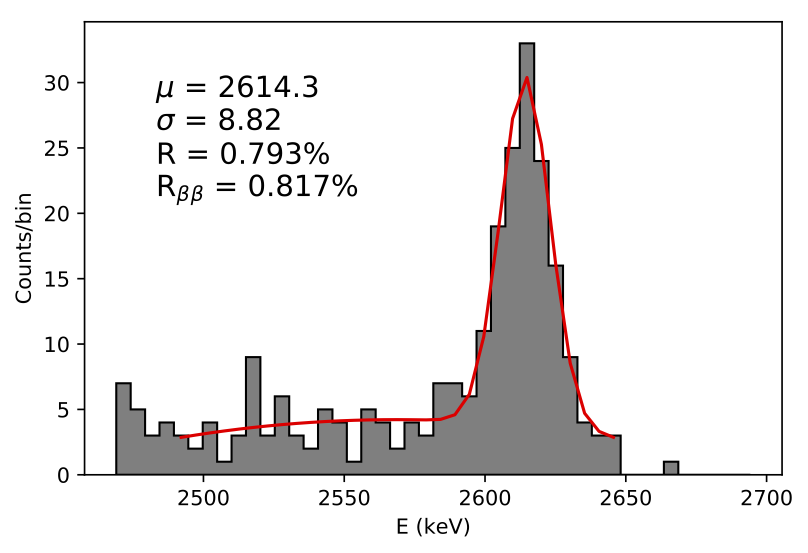
\includegraphics[width=0.25\textwidth]{moriond/CSTH_espectrum_Tl_photopeak_fit.png}
       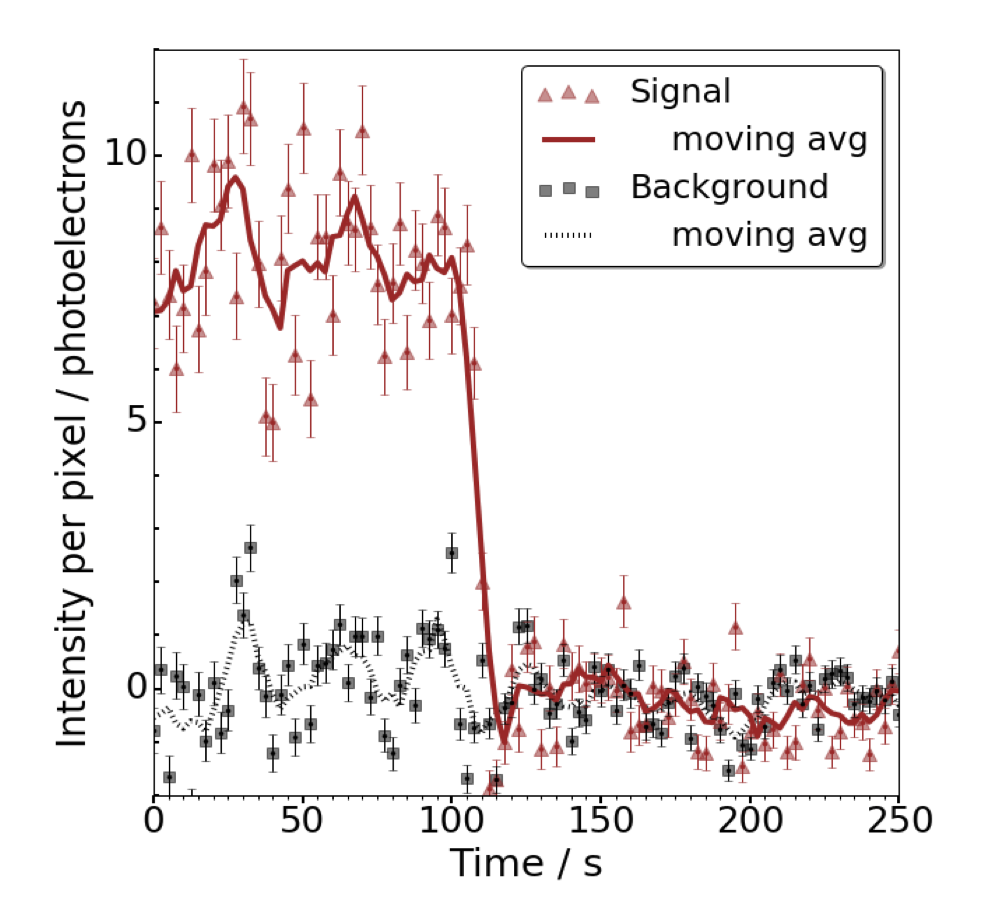
\includegraphics[width=0.20\textwidth]{moriond/smfi_trayectory.png}    
  \end{center}
 \end{figure}

 
\begin{itemize}
\item {\bf Topological signal}, capable to separate signal ``double electrons'', from backgrounds ``single electrons''. 
\item {\bf Excellent energy resolution}, 20 keV at \Qbb. 
\item {\bf Possibility to identify \Bapp} produced in $\XE \rightarrow \Bapp + 2 e (+ 2 \nu)$, through SMFI. 
\end{itemize}
\end{frame}


\begin{frame}
\frametitle{The NEXT program} 
 \begin{center}
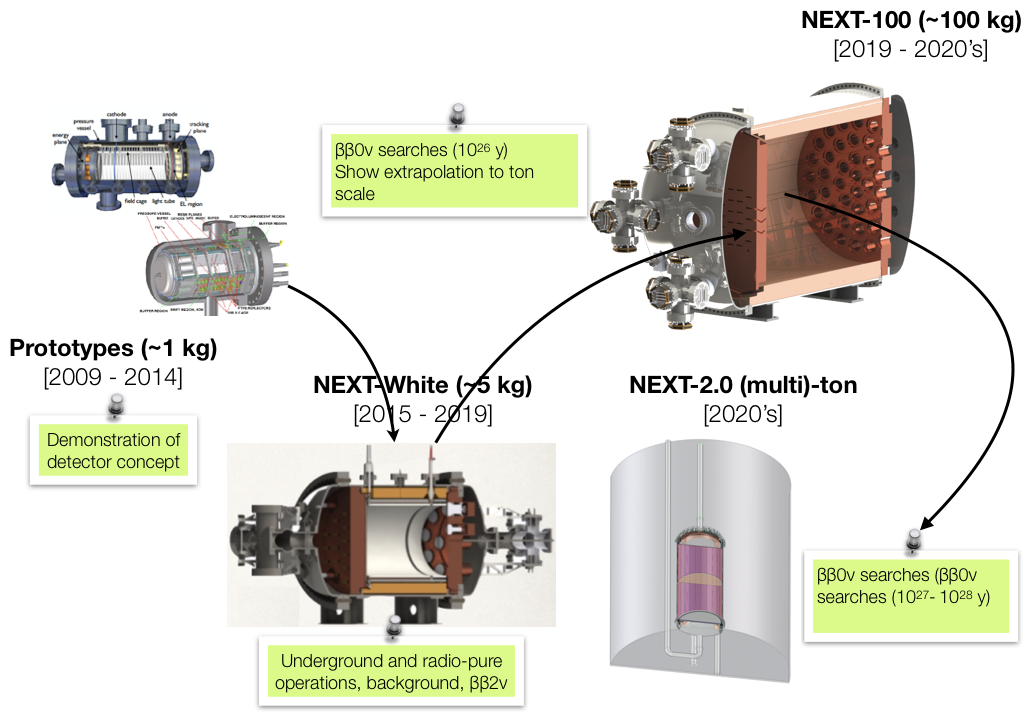
\includegraphics[width=0.85\textwidth]{moriond/next-program.png}
\end{center}
\end{frame}




\section{NEXT White (NEW)}
\begin{frame}
\frametitle{NEXT White (NEW)} 

 \begin{center}
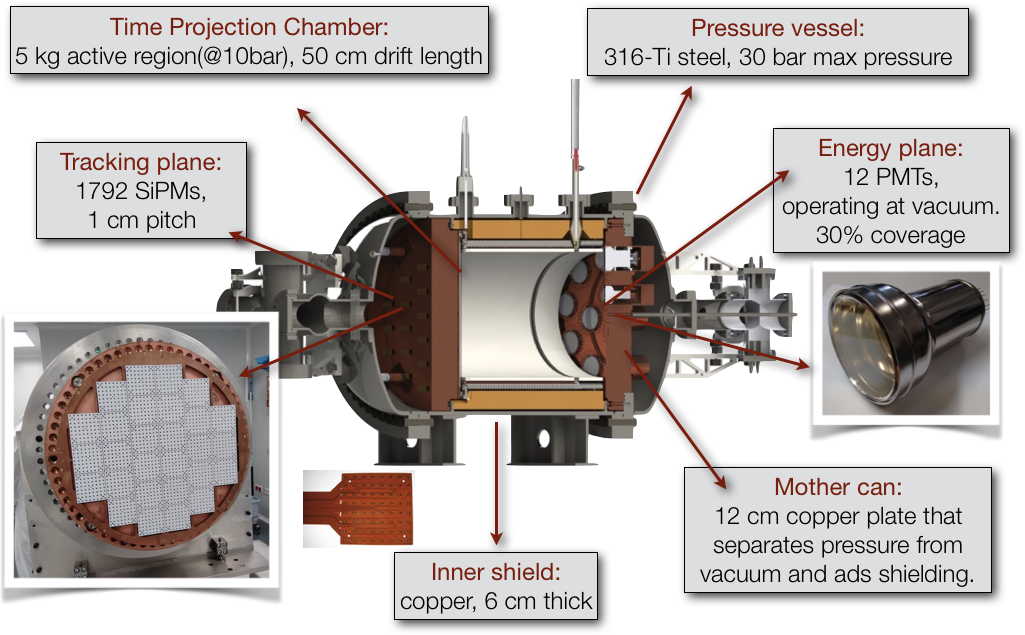
\includegraphics[width=0.85\textwidth]{moriond/next-white-drawing.png}
\end{center}
\end{frame}

\begin{frame}
 \begin{center}
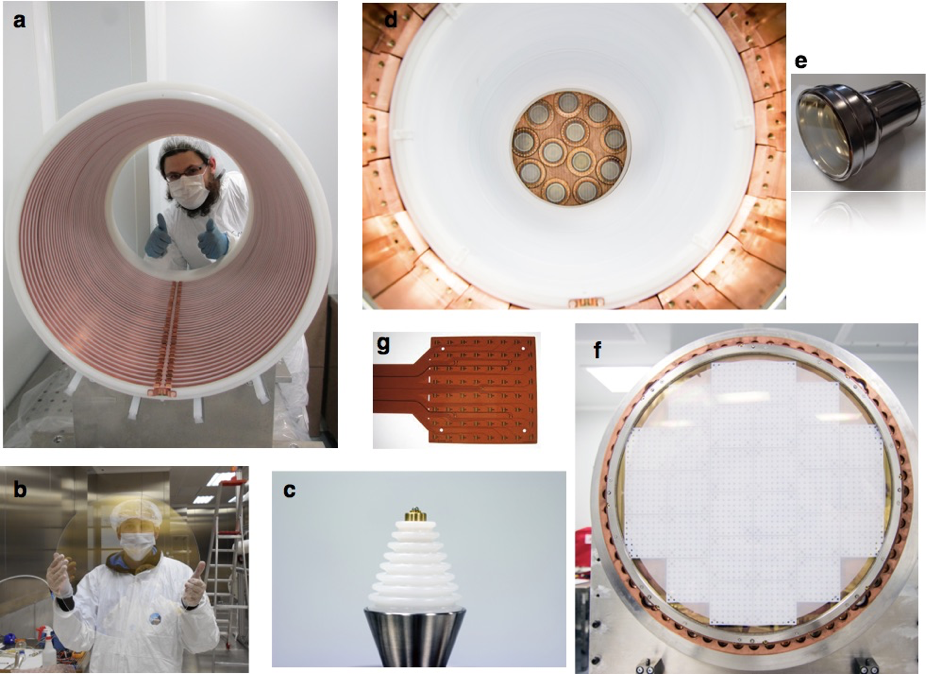
\includegraphics[width=0.85\textwidth]{moriond/next-parts.png}
\end{center}
\end{frame}

\begin{frame}
 \begin{center}
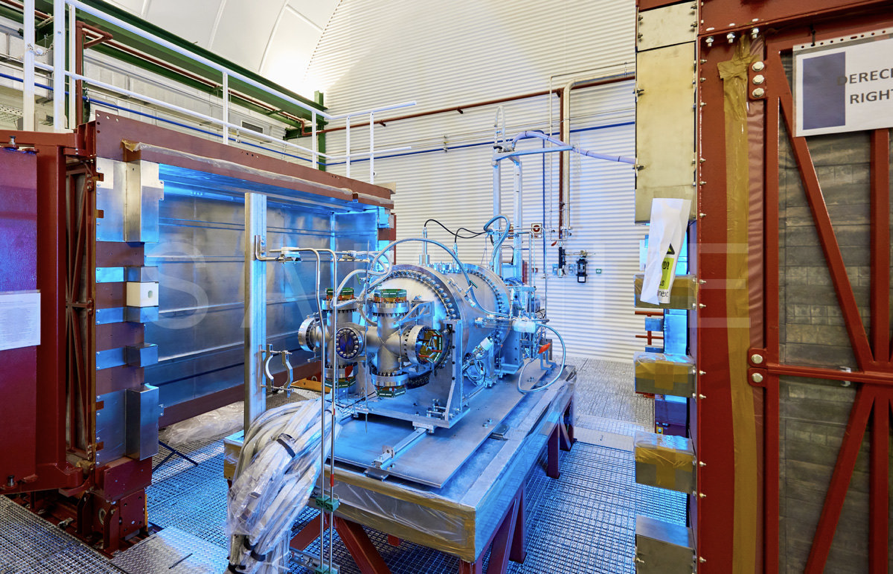
\includegraphics[width=0.85\textwidth]{moriond/next-white.png}
\end{center}
\end{frame}

\begin{frame}
\frametitle{Goals of NEW} 
\begin{itemize}
\item Demonstrate technology is robust. 
\item Demonstrate energy resolution and topological signature. 
\item Measure backgrounds to establish a reliable background model (and to improve it as needed). 
\end{itemize}
\end{frame}

\begin{frame}
\frametitle{Operation of NEW} 
 \begin{center}
 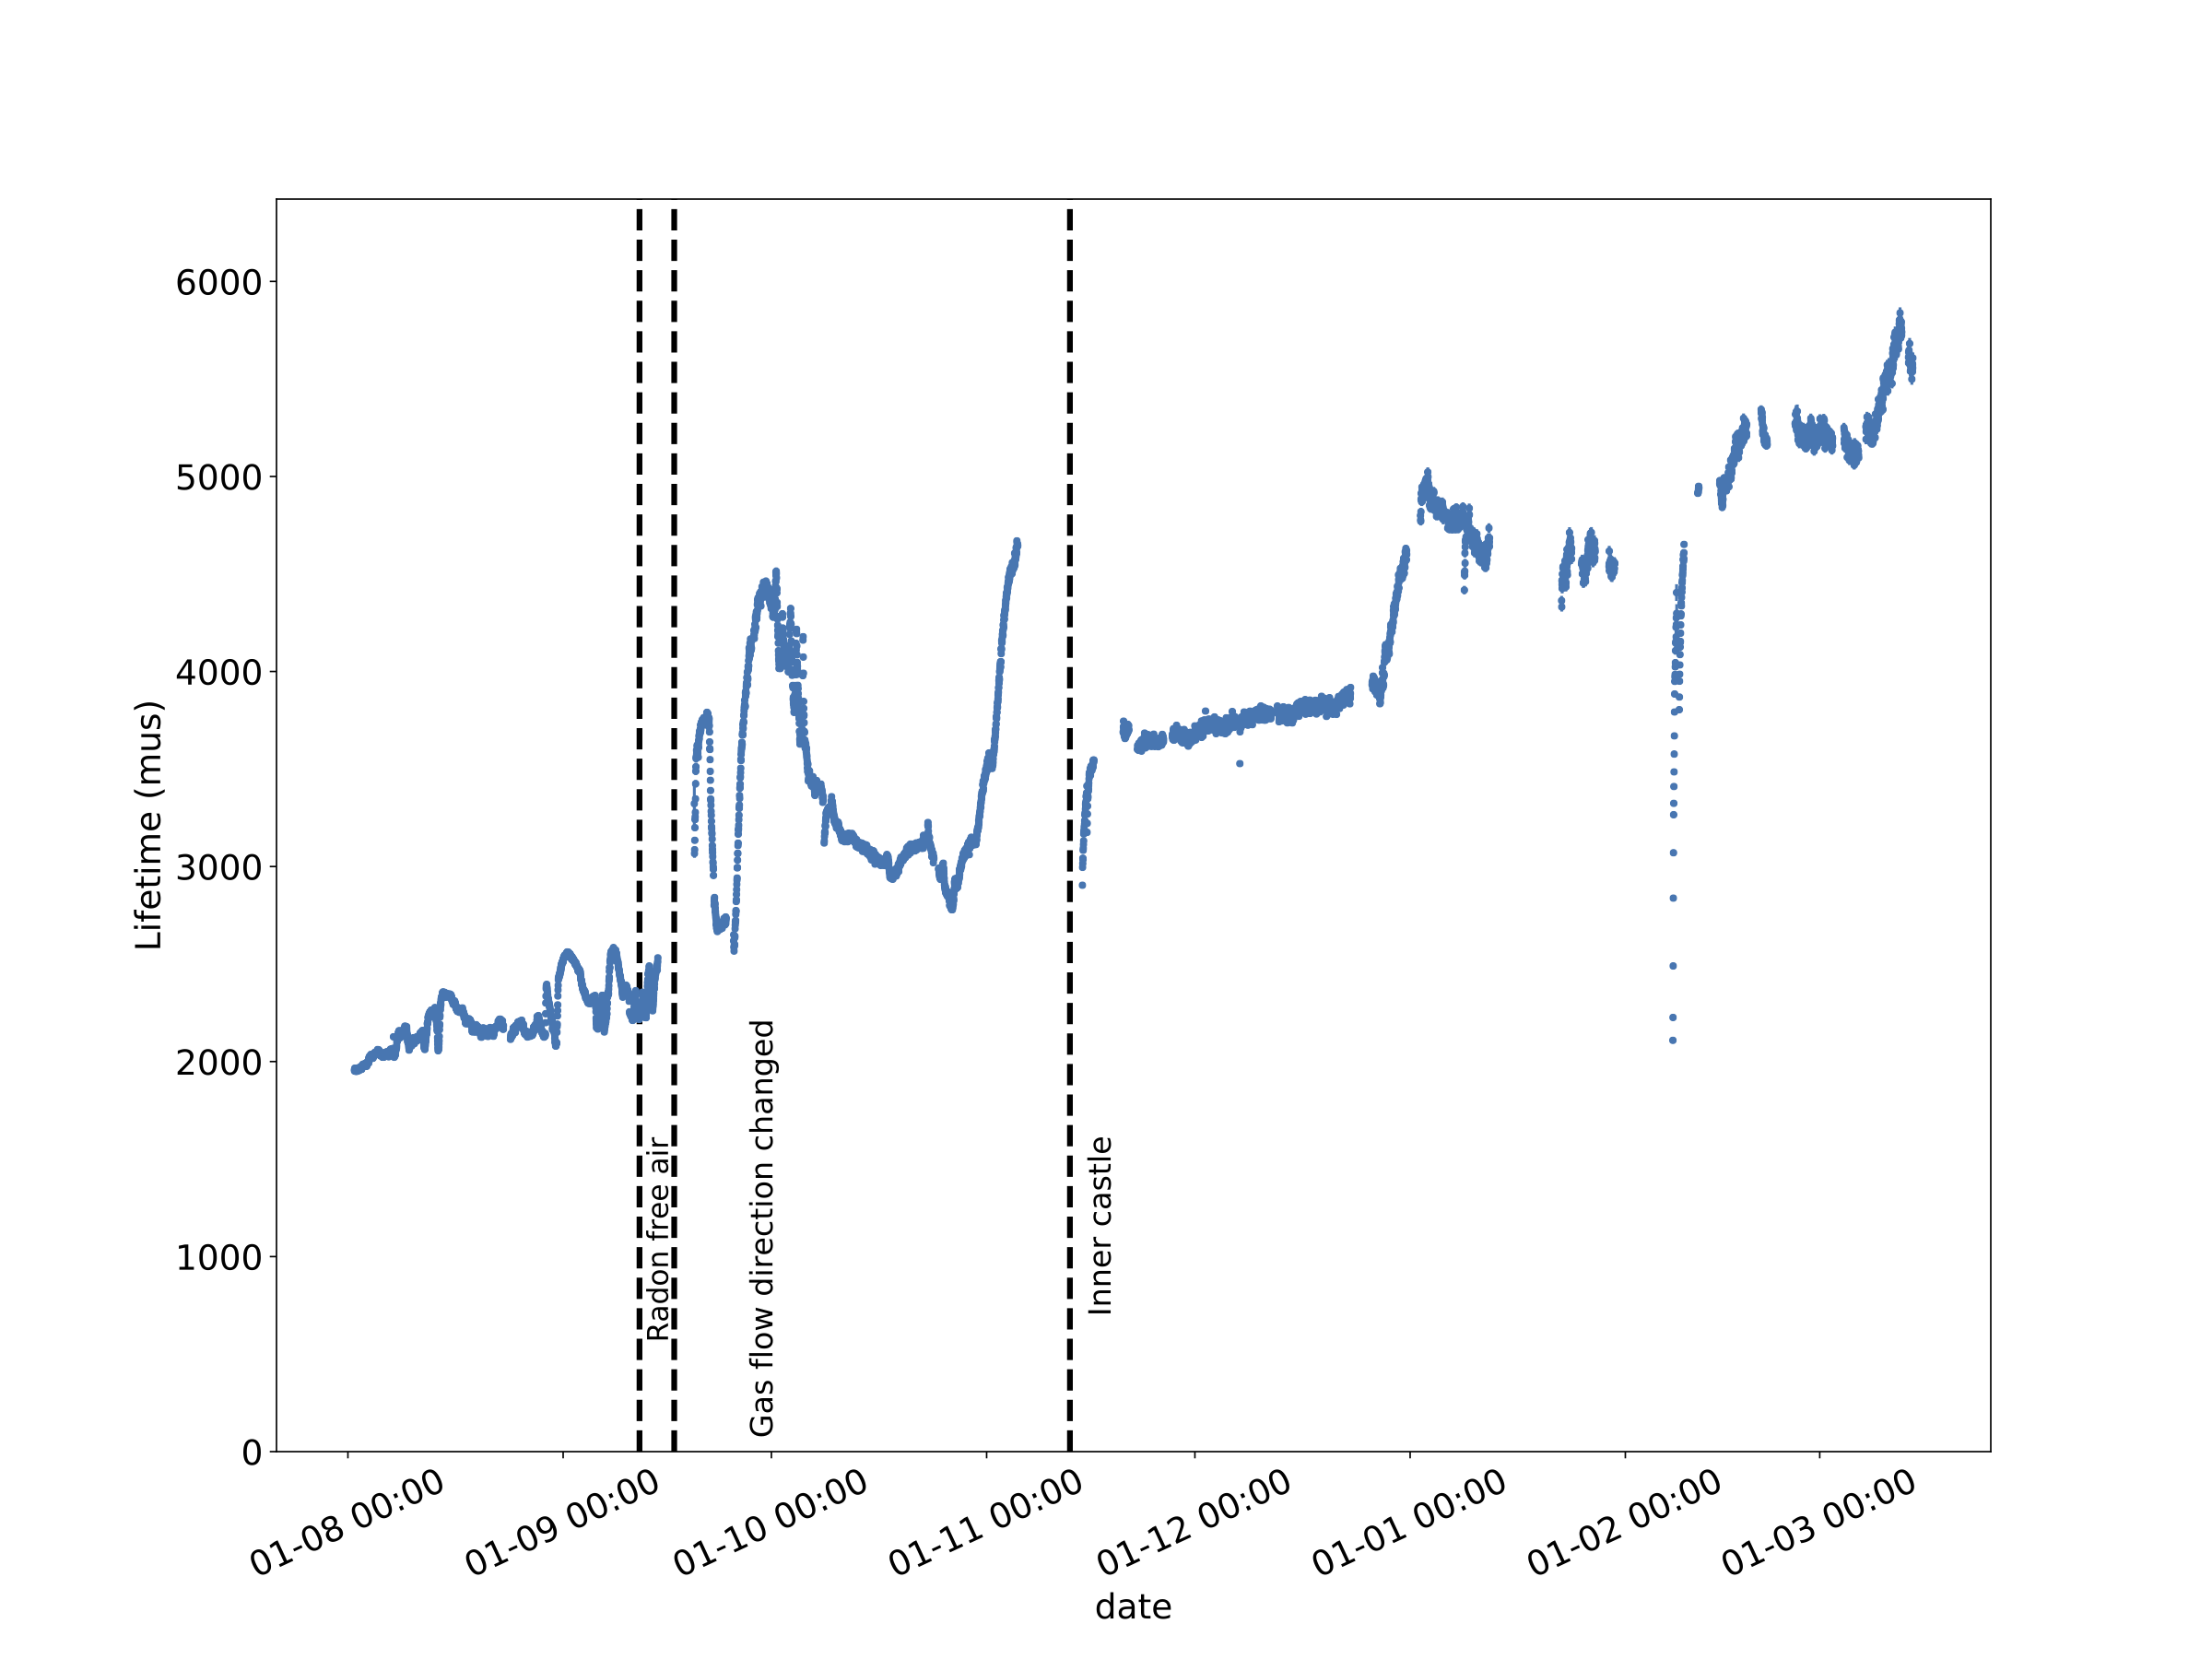
\includegraphics[width=0.65\textwidth]{moriond/lifetime_evolution.png}
\end{center}
\begin{itemize}
\item Taking data since 2016. Very stable operation since 2017.
\item Less than 1 gram of gas lost per year. 
\item Very high lifetime, measured on a daily basis with Krypton calibrations. 
\end{itemize}
\end{frame}

\begin{frame}
 \frametitle{NEW energy resolution} 
 \begin{center}
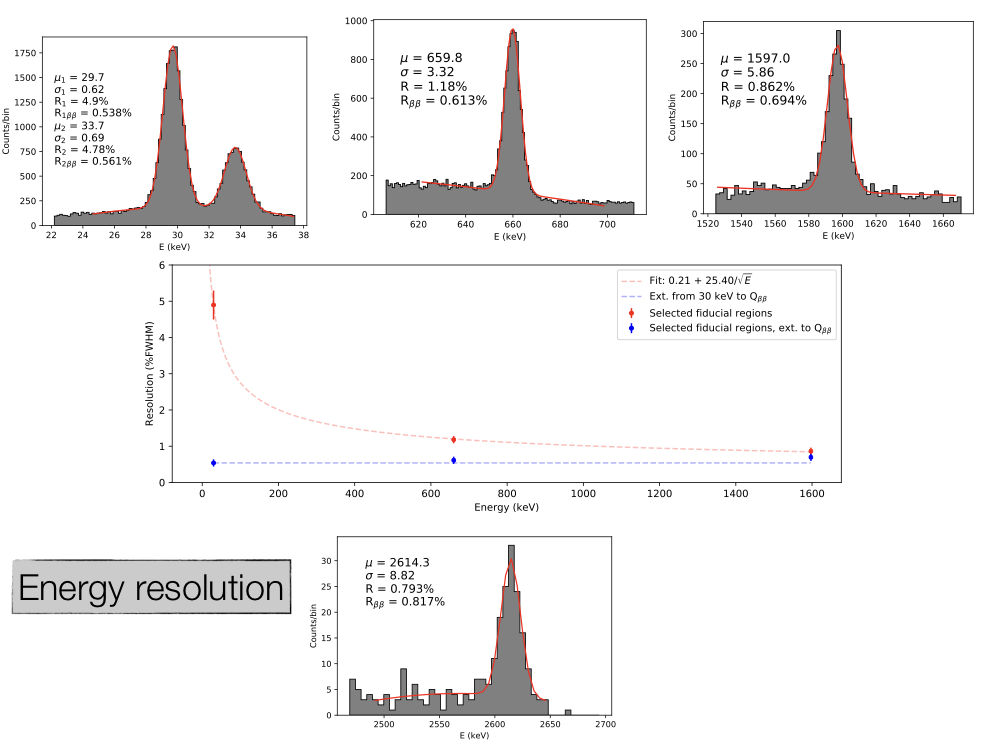
\includegraphics[width=0.85\textwidth]{moriond/new_energy_res.png}
\end{center}
\end{frame}

\begin{frame}
 \frametitle{NEW topological signature} 
 \begin{center}
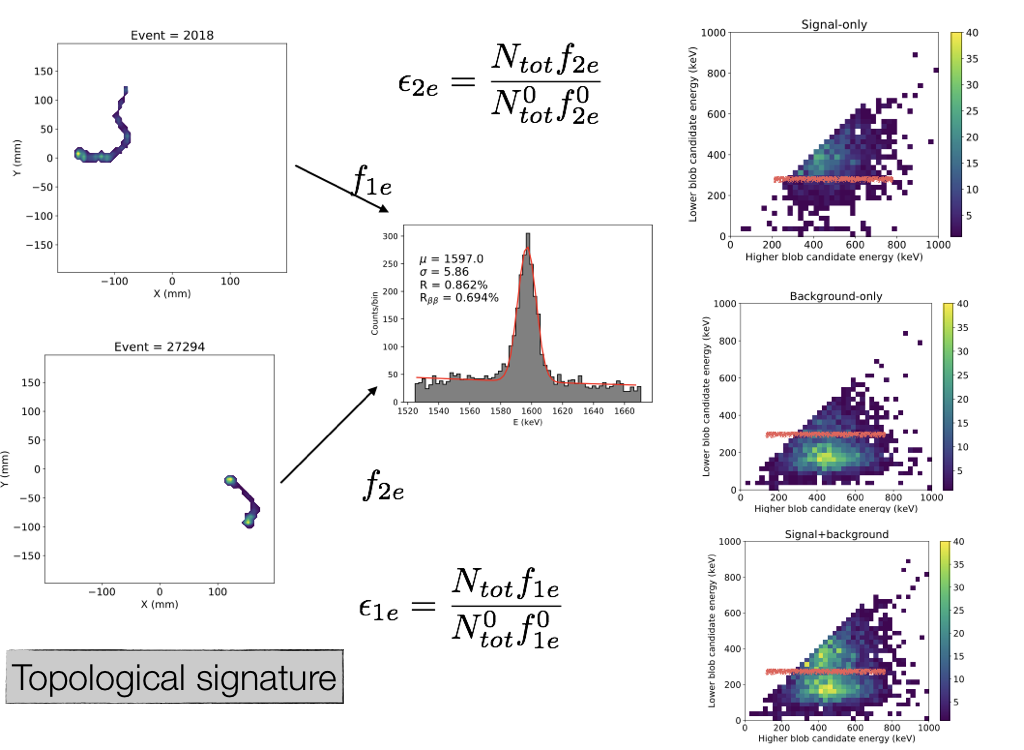
\includegraphics[width=0.85\textwidth]{moriond/new_topo_doublescape.png}
\end{center}
\end{frame}

\begin{frame}
 \begin{center}
 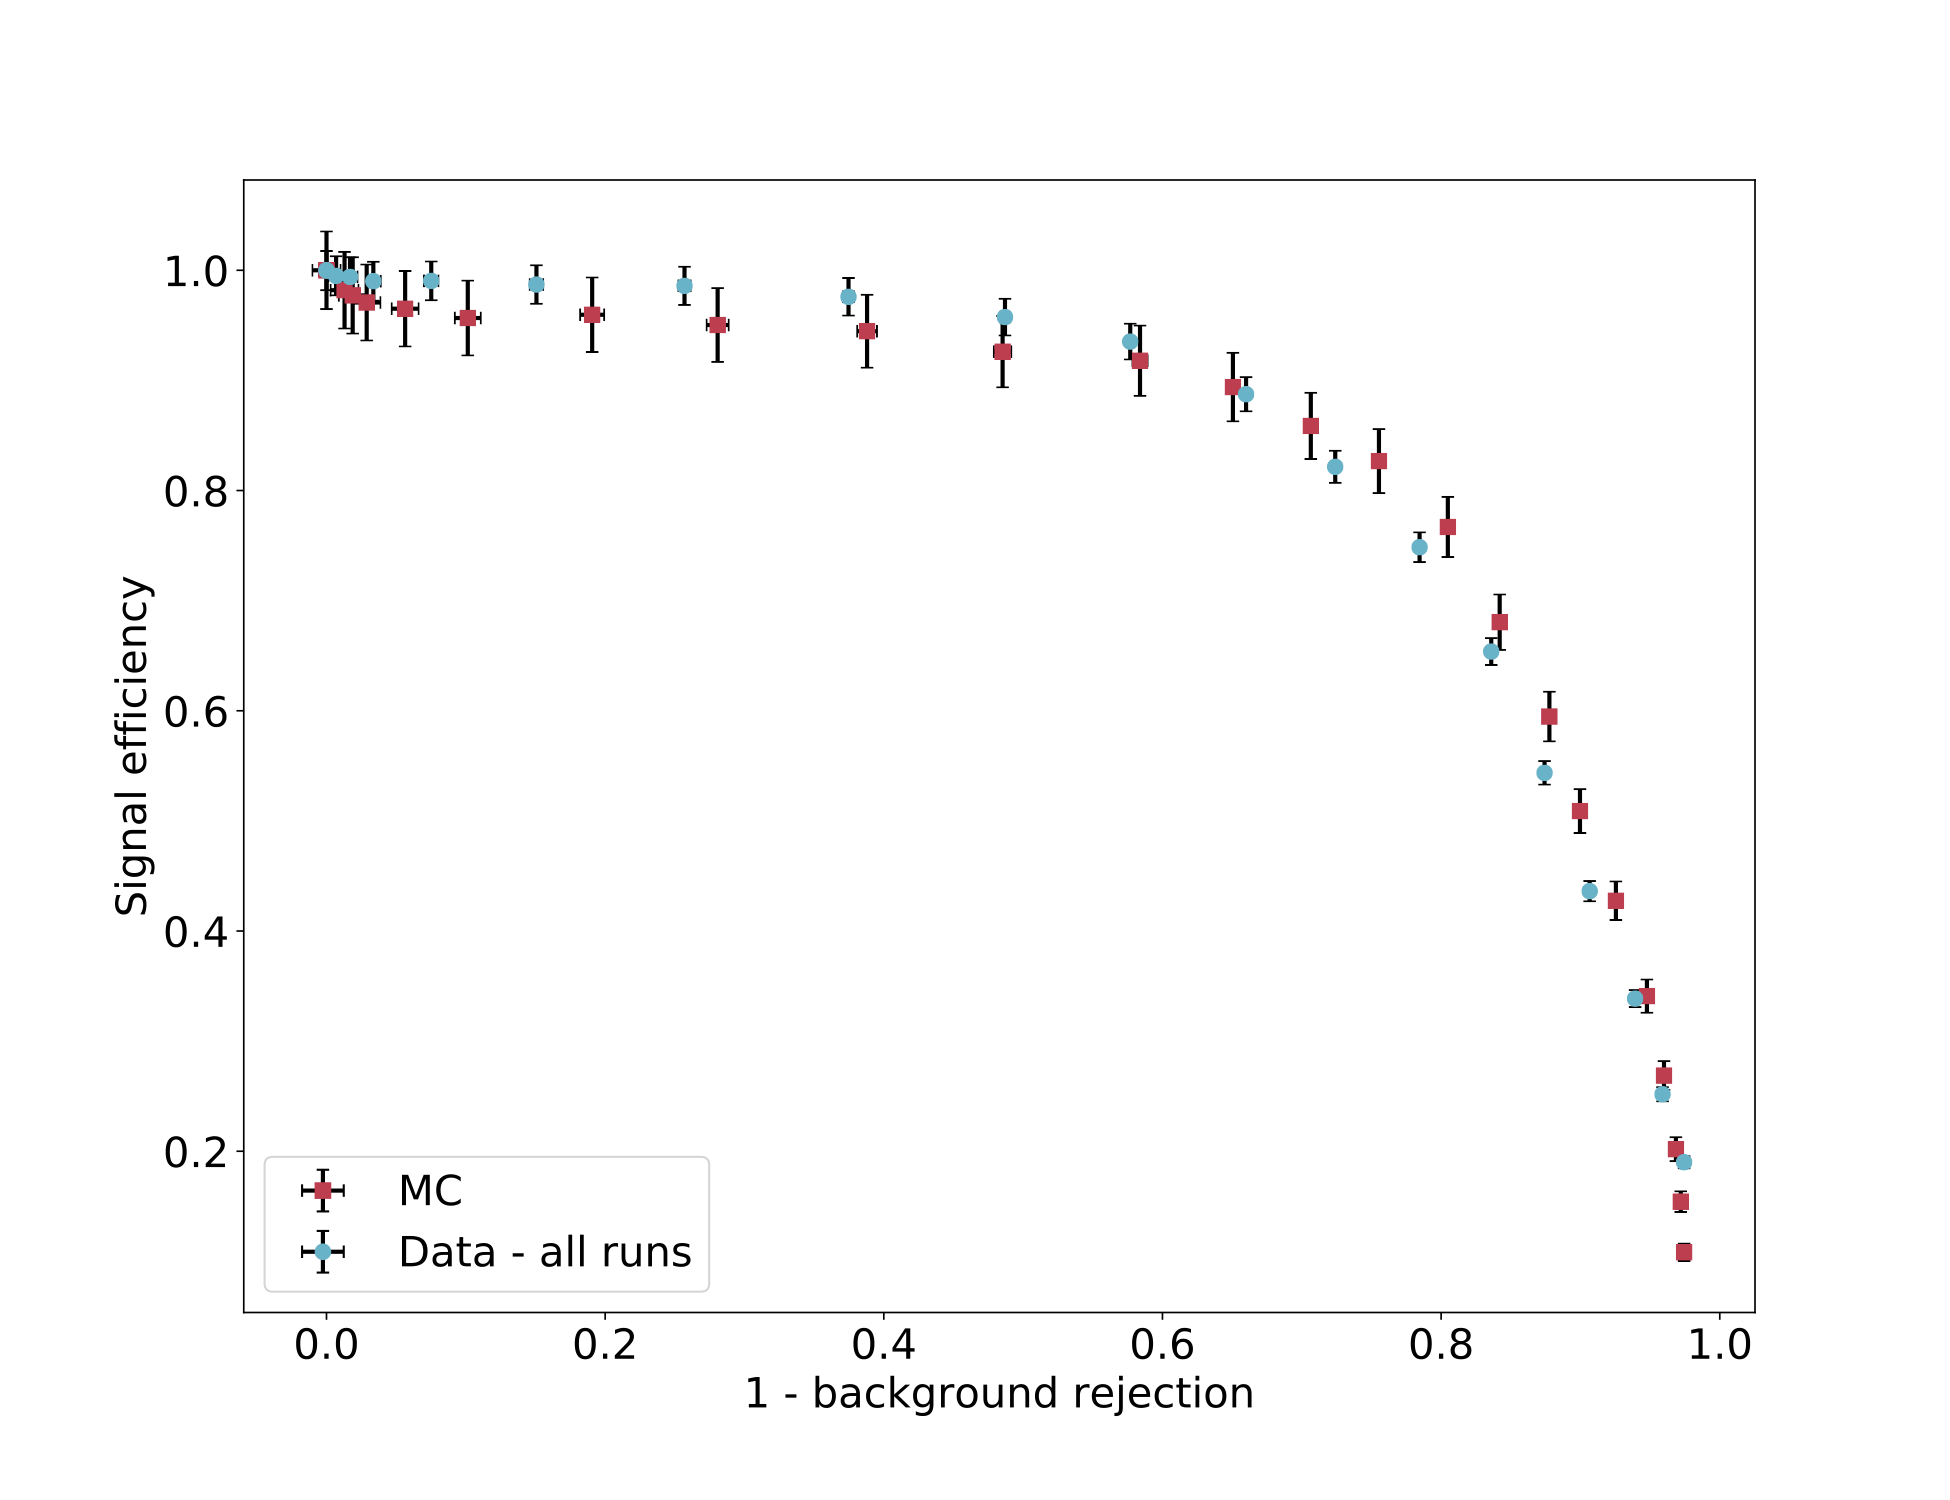
\includegraphics[width=0.45\textwidth]{moriond/new_topo_data_mc.png}
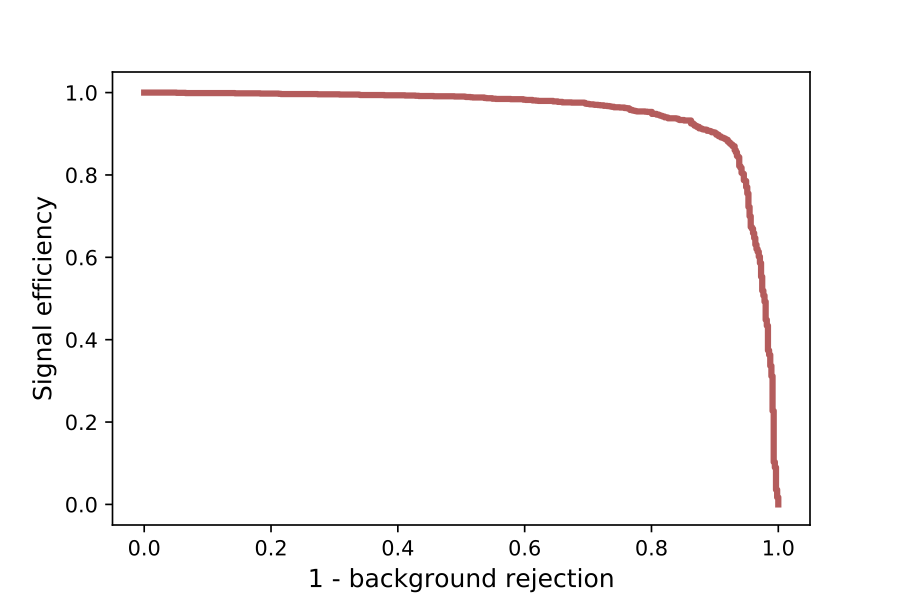
\includegraphics[width=0.50\textwidth]{moriond/eff_vs_bkg_dnn.png}
\end{center}

\begin{itemize}
\item {\bf Blob analysis}, in \TL\ double escape peak shows good agreement data/MC. 
\item {\bf DNN analysis}, optimizes separation signal/background. Shown MC prediction: 90 \% signal efficiency 10\% background contamination. 
\end{itemize}
\end{frame}






\section{Background measurement in \NEW}


\begin{frame}
\frametitle{Background measurements (Run IV, 2018)} 
\begin{figure}
  \begin{center}
    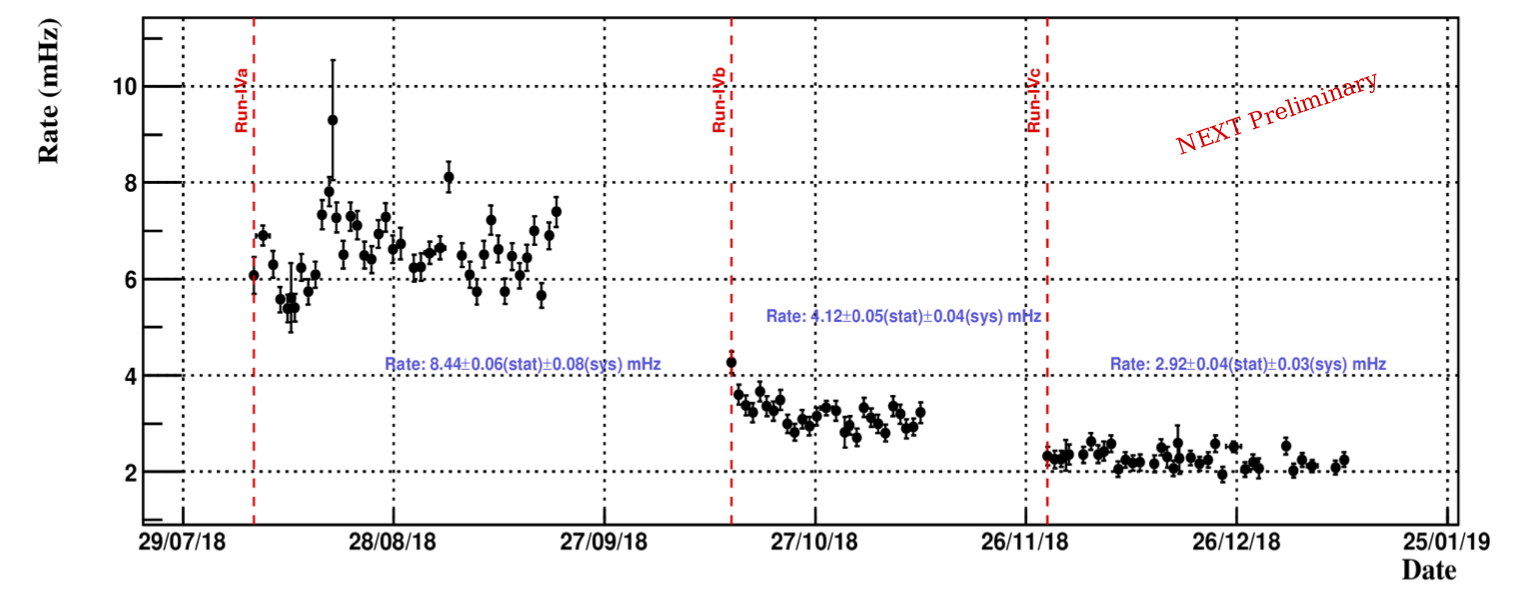
\includegraphics[scale=0.4]{moriond/run4_fid_rate.png}
    \caption{Fiducial background rate for Run IV (2018) as a function of data taking calendar day. Vertical dashed lines mark the times where Run-IVa, Run-IVb and Run-IVc started.}
    \label{fig:rate}
  \end{center}
\end{figure}
\begin{itemize}
\item {\bf Run IVa}. No radon free air, no inner shielding. 
\item {\bf Run IVb}. Radon free air. 
\item {\bf Run IVc}. Radon free air and inner shielding
\end{itemize}
\end{frame}

\begin{frame}
\frametitle{Background composition} 
\begin{figure}
  \begin{center}
    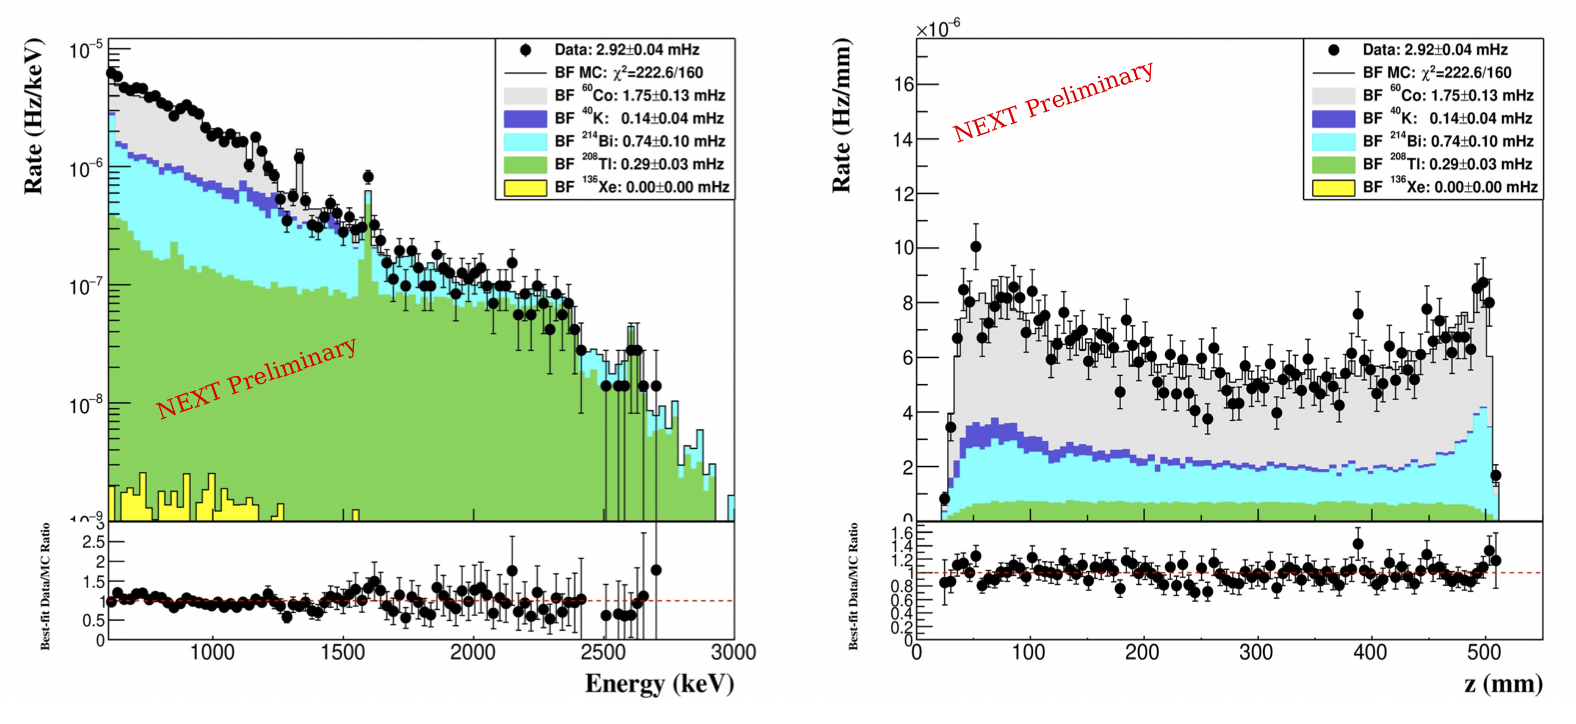
\includegraphics[scale=0.4]{moriond/bkgnd_fit.png}
    \caption{Contribution of the dominant background isotopes to \NEW\ radioactive budget.}
    \label{fig:rate}
  \end{center}
\end{figure}
\begin{itemize}
\item Notice, only \BI\ and \TL\ relevant for \bbonu\ searches. 
\end{itemize}
\end{frame}

%\begin{frame}
%\frametitle{Background composition (Run IV)} 
%\begin{figure}
%  \begin{center}
%    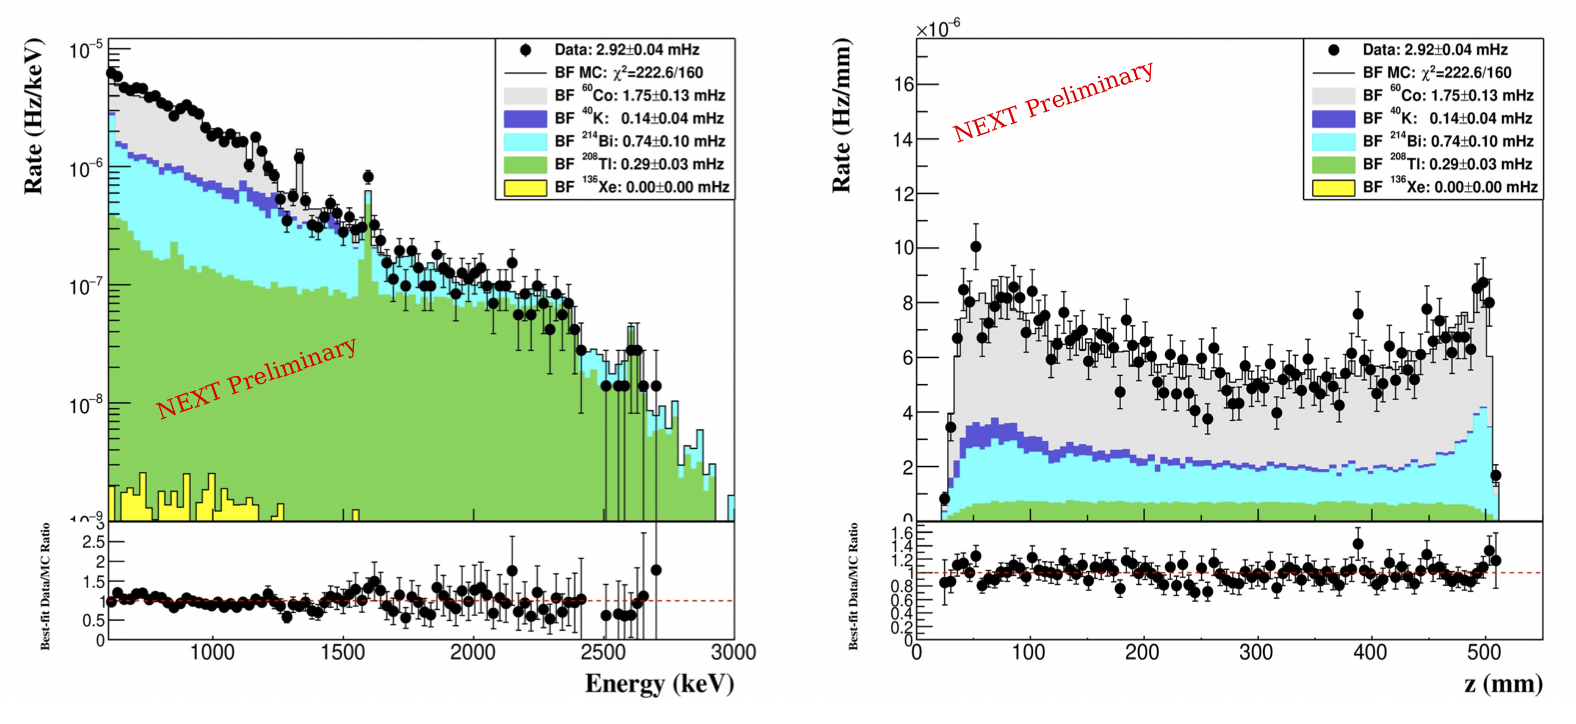
\includegraphics[scale=0.4]{moriond/bkgnd_fit.png}
%    \caption{Contribution of the dominant background isotopes to \NEW\ radioactive budget.}
%    \label{fig:rate}
%  \end{center}
%\end{figure}
%\begin{itemize}
%\item Notice, only \BI\ and \TL\ relevant for \bbonu\ searches. 
%\end{itemize}
%\end{frame}


\begin{frame}
\frametitle{Run V (enriched xenon)} 
\begin{figure}
  \begin{center}
    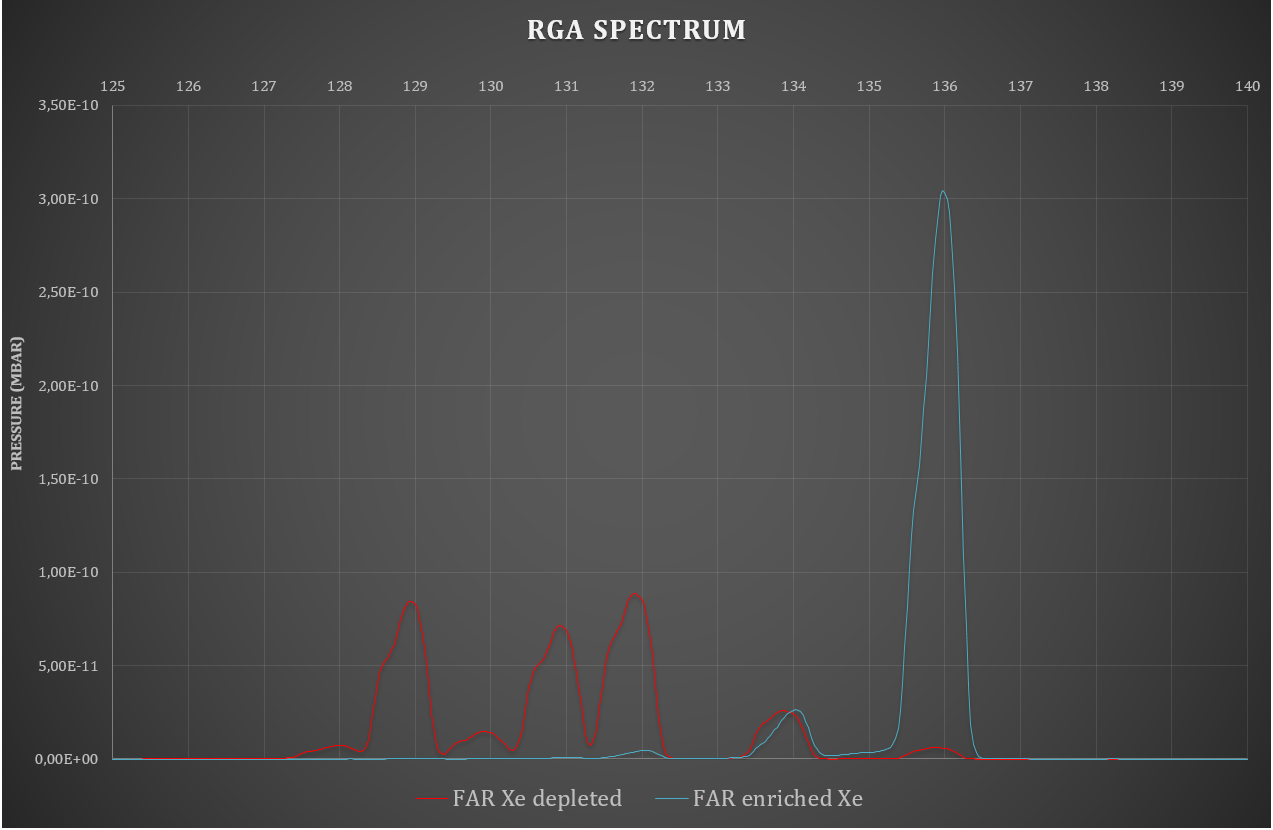
\includegraphics[width=0.9\textwidth]{moriond/XeEnriched.png} 
    \caption{We really have enriched xenon...}
    \label{fig:exe}
  \end{center}
\end{figure}
\end{frame}

\begin{frame}
\frametitle{Measurement of \bbtnu\ mode (Run V)} 
\begin{figure}
  \begin{center}
    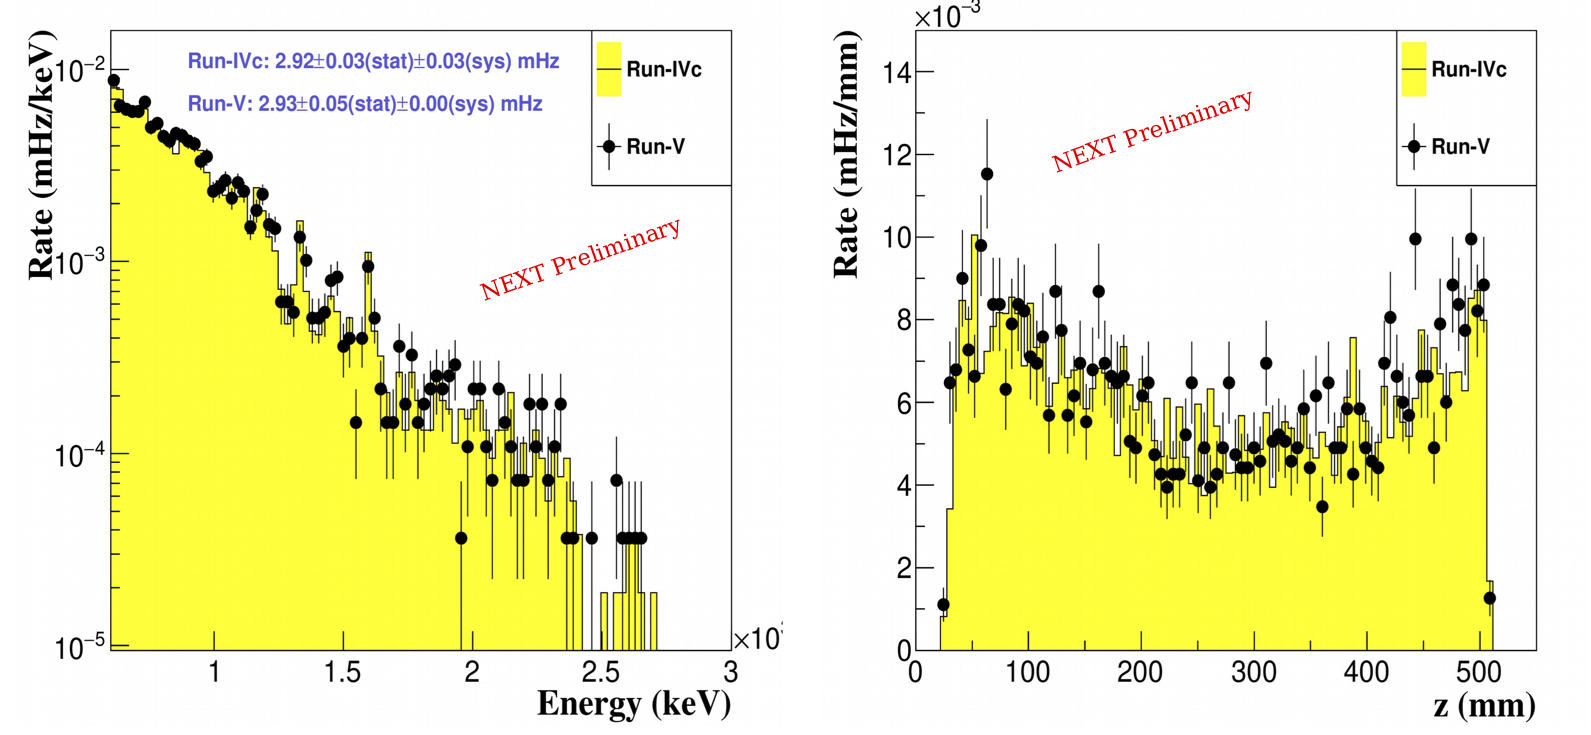
\includegraphics[scale=0.4]{moriond/run5_spectra.png}
    \caption{Energy spectra, Run V.}
    \label{fig:rate}
  \end{center}
\end{figure}
\begin{itemize}
\item Notice, Run V just started (15 days taking data with enriched xenon). 
\item Will run until the end of the year to provide a measurement of \bbtnu\ lifetime.  
\end{itemize}
\end{frame}

\begin{frame}
\frametitle{High energy spectrum with topological cuts} 
\begin{figure}
  \begin{center}
    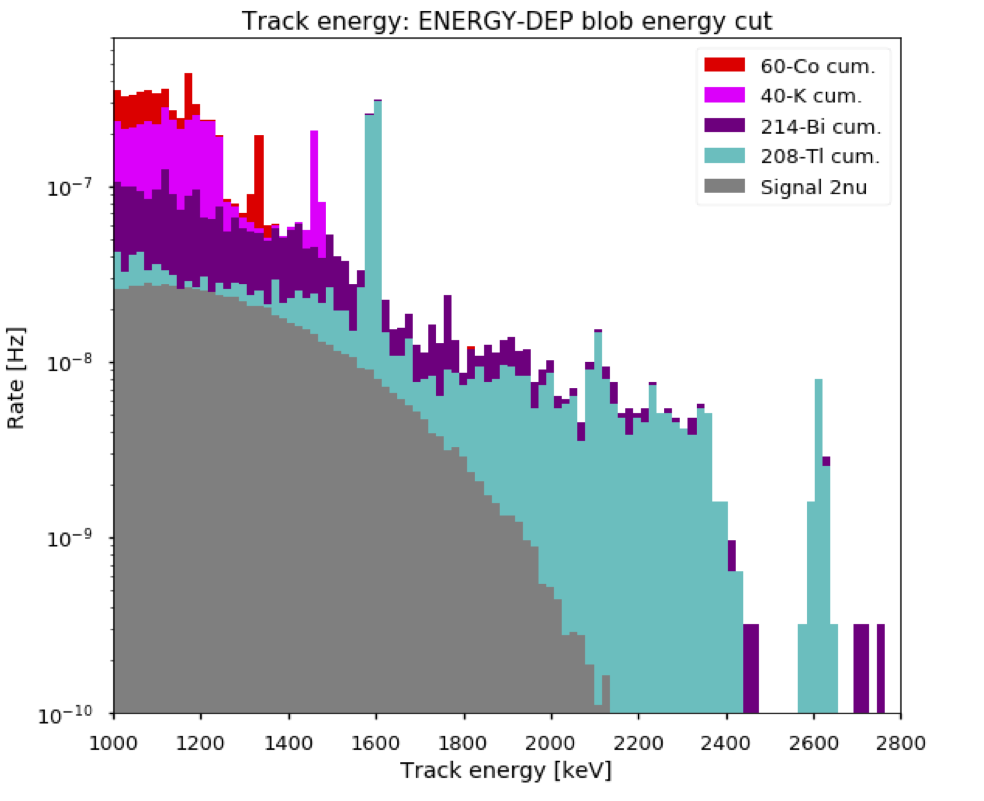
\includegraphics[scale=0.35]{moriond/new_with_topo_log.png}
     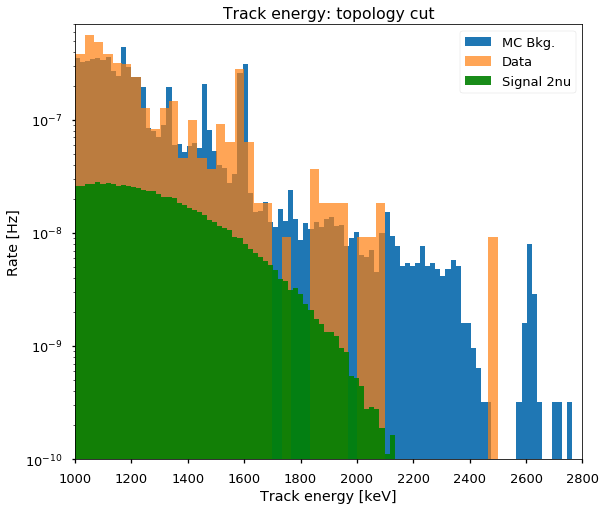
\includegraphics[scale=0.30]{moriond/energy_spectrum_total.png}
    
    \caption{Energy spectra with topological cuts data and MC. }
    \label{fig:rate}
  \end{center}
\end{figure}
\begin{itemize}
\item Topological cut cleans high energy region where signal is expected (notice the hole). 
\item One candidate event found in the data by basic topological analysis (visual inspection shows badly reconstructed single electron event).  
\end{itemize}
\end{frame}





%\begin{frame}
%\begin{table}[!htb]
%\caption{\label{tab:rate} Run-IV background rates for events with energy above 600 keV.}
%\begin{center}
%\begin{tabular}{ccc}
%\hline
%Run period & Inclusive rate (mHz) & Fiducial rate (mHz) \\ \hline
%Run-IVa    &    14.85$\pm$0.06    &  7.05$\pm$0.05                  \\ 
%Run-IVb    &     8.77$\pm$0.06    &  3.70$\pm$0.04                  \\
%Run-IVc    &     7.03$\pm$0.10    &  2.72$\pm$0.06                   \\ \hline
%\end{tabular}
%\end{center}
%\end{table}
%\end{frame}
%
%\begin{frame}
%\begin{figure}
%  \begin{center}
%    \includegraphics[scale=0.6]{img2/RateTime_eFidSel_RunIVabc.pdf}
%    \caption{Fiducial background rate as a function of data taking calendar day. Vertical dashed lines mark the times where Run-IVa, Run-IVb and Run-IVb started.}
%    \label{fig:rate}
%  \end{center}
%\end{figure}
%\end{frame}
%
%\begin{frame}
%\begin{figure}
%  \begin{center}
%    \includegraphics[scale=0.40]{img2/RunIVabc_energy.pdf}
%    \caption{Fully corrected energy spectra of the fiducial background samples collected during Run-IV.}
%    \label{fig:energy}
%  \end{center}
%\end{figure}
%\end{frame}
%
%\begin{frame}
%\frametitle{Run-IVa} 
%\begin{itemize}
%\item The background rate in Run-IVa has decreased by a factor of 1.7 with respect to the earlier pilot background run taken in 2017 (Run-II), despite the pressure increase from 7.2 to 10 bar.
%\item This background rate reduction confirms the expected improvement in detector radiopurity introduced by the replacement of the field cage resistor chain and the PMT bases in early 2018.
%\item However, the rate variations in time (not consistent with statistical fluctuations) observed for Run-IVa in Fig.~\ref{fig:rate} are a clear indication of a time-dependent background source, thereby not related to radio-impurities of the detector materials.
%\item The analysis of the correlation of the background rate with the level of airborne radon at the LSC has allowed to conclude that such variations are due to a significant contribution of $^{222}$Rn decays within the volume of the lead castle.  
%\item Using the radon activity data provided by the Alphaguard detector, the correlation is quantified in Fig.~\ref{fig:rncorr} by means of a linear fit. From this fit, an expectation of the fiducial background rate in NEXT-White for a zero-Rn-activity is derived: 3.65$\pm$0.37 mHz.    
%\end{itemize}
%\end{frame}
%
%\begin{frame}
%\begin{figure}
%  \begin{center}
%    \includegraphics[scale=0.64]{img/RnCorr_eFidSel.eps}
%    \caption{Airborne radon activity versus Run-IVa fiducial background rate. A linear fit extrapolation to zero-Rn-activity yields an expected background rate of 3.65$\pm$0.37 mHz.}
%    \label{fig:rncorr}
%  \end{center}
%\end{figure}
%\end{frame}
%
%\begin{frame}
%\frametitle{Run-IVb} 
%\begin{itemize}
%\item The effect of the RAS in Run-IVb is clearly visible in Fig.~\ref{fig:rate} and Fig.~\ref{fig:energy}. After a few-days period where the background rate decreases as the remaining $^{222}$Rn inside the castle decays, the fiducial background rate becomes stable when a reduction of a factor of 1.9 with respect to Run-IVa is reached.
%\item The comparison of the energy spectra in Run-IVa and Run-IVb around 1700 keV (1764 keV $\gamma$-line of $^{214}Bi$) positively identifies this reduction as due to $^{222}$Rn.
%\item The consistency between the background rate measurement in Run-IVb (3.70$\pm$0.04 mHz) and the zero-Rn-activity background extrapolation from Run-IVa (3.65$\pm$0.37 mHz) implies that the RAS allows for a virtually airborne-Rn-free operation of the NEXT-White detector. 
%\end{itemize}
%\end{frame}
% 
% \begin{frame}
%\frametitle{Run-IVc} 
%\begin{itemize}
%\item The main goal of the ILC installed between Run-IVb and Run-IVc is to provide further shielding to background contributions coming from the outer lead castle volume. 
%\item In particular, the radioactivity from the castle structure paint is a major candidate to be suppressed.
%\item As shown, Fig.~\ref{fig:rate} and Fig.~\ref{fig:energy}, the Run-IVc data already indicates a reduction in the fiducial background rate of about 40\% despite the current limited statistics. 
%\item This implies that Run-IVa and Run-IVb suffer from a significant contribution of external backgrounds not related to airborne radon ($\sim$1 mHz). The main candidate source of this external background is the castle structure paint.
%\item Beyond the reduction of overall background rate, it is worth remarking the stability of the rate over time, presented in Fig.~\ref{fig:ratec}. 
%\end{itemize}
%\end{frame}
%  
% \begin{frame}
%\begin{figure}
%  \begin{center}
%    \includegraphics[scale=0.60]{img2/Rate_eFidSel_time.pdf}
%    \caption{Run-IVc fiducial background rate as a function of calendar day. A linear fit shows the compatibility with a flat distribution. The vertical dashed lines marks the time of the different sub-runs taken so far.}
%    \label{fig:ratec}
%  \end{center}
%\end{figure}
%\end{frame}
%%
%%
%\begin{frame}
%\frametitle{Background model} 
%\begin{itemize}
%\item The expected background budget in NEXT-White is derived from a detailed background model accounting for different isotopes and detector volumes. 
%\item The model relies on the extensive radiopurity measurements campaign conducted by the NEXT collaboration. Up to 41 detector materials have been considered, screening their $^{214}$Bi, $^{208}$Tl, $^{40}$K and $^{60}$Co contributions.
%\item According to these measurements, a full GEANT4-based Monte-Carlo simulation has been performed. The screened materials are associated to 19 GEANT-4 volumes describing the components of the NEXT-White detector. These volumes can be grouped in 6 different detector subsystems: active volume, energy readout plane, tracking readout plane, field cage, pressure vessel and shielding. Accounting for the 4 isotopes considered, the background model consists of 76 (19$\times$4) background sources. In addition, the contribution from the $\beta\beta2\nu$ of $^{136}$Xe, whose fraction in the depleted Xe in use is 2.86\%, is also incorporated to the model. Overall, 10$^{11}$ background events have been simulated, corresponding to an exposure of 6.35 year. 
%\end{itemize}
%\end{frame}
%
%\begin{frame}
%\begin{itemize}
%\item The simulated background events are first processed to mimic the electronic effects (readout, shaping, noise, ...), so the corresponding raw waveforms can be already compared to the ones collected by the DAQ system. Then, the Monte-Carlo events are passed through the same reconstruction and corrections steps as described for real data. Finally, the fiducial selection is applied. 
%\item The resulting background energy spectra are shown in Fig.~\ref{fig:bgmodel}, in terms of the different isotopes contribution (right) and of the different subsystem contributions (left). Since the background model includes neither the contribution of external airborne-Rn nor the ILC, it is to be compared with the data taken in Run-IVb. According to the described model, the expected fiducial background rate in Run-IVb is 1.699$\pm$0.003 (stat) mHz.
%\item An updated background model is being currently built considering the ILC, thus to be compared with the Run-IVc data. In particular, the $^{214}$Bi, $^{208}$Tl, $^{40}$K and $^{60}$Co contributions of the ILC bricks, as well as the $^{214}$Bi and $^{208}$Tl contribution of the ILC steel structure, are accounted for. In addition, a new contribution from Rn-induced $^{214}$Bi on the cathode surface is included, according to the measurements performed with Run-II data. Overall, the updated model consists of 84 background sources. So far, 1.5 million events (corresponding to 5.48 years) have been simulated and are currently being processed in the reconstruction stage. 
%\end{itemize}
%\end{frame}
%
%\begin{frame}
%\begin{figure}
%  \begin{center}
%    \includegraphics[scale=0.3]{img/MCE.eps}
%    \includegraphics[scale=0.3]{img/MCEVol.eps}
%    \caption{MC background model for Run-IVb: fiducial background rate as a function of the energy. Right: contributions from the 4 isotopes considered. Left: contributions from the 6 subsystems considered, accounting for 19 GEANT-4 volumes.}
%    \label{fig:bgmodel}
%  \end{center}
%\end{figure}
%\end{frame}
%
%\begin{frame}
%\frametitle{Data-Monte Carlo comparison} 
%\begin{itemize}
%\item The comparison of the background model described previously with the Run-IVb data is presented in the left panel of Fig.~\ref{fig:bgfit}. While the different gamma lines are well reproduced in the model, the overall data rate (3.70$\pm$0.04) deviates from the expectation (1.699$\pm$0.003 mHz) by a factor $\sim$2.2 It is worth noticing that a good fraction of such a discrepancy is due to external backgrounds that have been suppressed in Run-IVc with the ILC. {\em This consideration, along with the missing contribution of Rn-induced $^{214}$Bi on the cathode in the current model, allows to foresee a good matching between the data and the model in the near-future Run-IVc comparison}. 
%\item In order to tune the Run-IVb background model so it matches the data, an effective fit has been performed. The fit consists of the minimization of a maximum extended likelihood, considering both the energy and the z-coordinate distribution of the background events, as well as three effective background volumes in the model. The three volumes account for all materials in the anode and cathode regions, and in any other region (ie, field cage, vessel, and shielding). The rationale for the definition of these effective volumes is to fully exploit the clear z-dependence observed in the background data. 
%\item The best-fit reproduces the energy spectrum, although yielding an overall scale factor of the expected rate of 2.19$\pm$0.15. 
%\end{itemize}
%\end{frame}
%
%\begin{frame}
%\begin{figure}
%  \begin{center}
%    \includegraphics[scale=0.30]{img/DataMCE_eFidSel_EZFit_3Vols.eps}
%    \includegraphics[scale=0.30]{img/DataMCEBF_eFidSel_EZFit_3Vols.eps}
%    \caption{Fiducial background energy spectra in Run-IVc. Data (black dots) are superimposed to the background model expectation (solid histograms), for which the different isotopes contributions are shown. Left: expectation from nominal background model. Right: expectation from best-fit to data, were the displayed best-fit values correspond to the scale factor of each isotope with respect to the nominal model.}
%    \label{fig:bgfit}
%  \end{center}
%\end{figure}
%\end{frame}
%
%\begin{frame}
%\begin{figure}
%  \begin{center}
%    \includegraphics[scale=0.30]{img/DataMCZBF_eFidSel_EZFit_3Vols.eps}
%    \includegraphics[scale=0.30]{img/DataMCRBF_eFidSel_EZFit_3Vols.eps}
%    \caption{Fiducial background spatial distribution in Run-IVc. Data (black dots) are superimposed to the best-fit background model expectation (solid histograms), for which the different isotopes contributions are shown. Left: z distribution. Right: radial distribution. The displayed best-fit values correspond to the scale factor of each isotope with respect to the nominal model.}
%    \label{fig:zrbgfit}
%  \end{center}
%\end{figure}
%\end{frame}
%
 

\section{NEXT-100}
\begin{frame}
\frametitle{NEXT-100}

\begin{figure}[tbh!]
  \begin{center}
      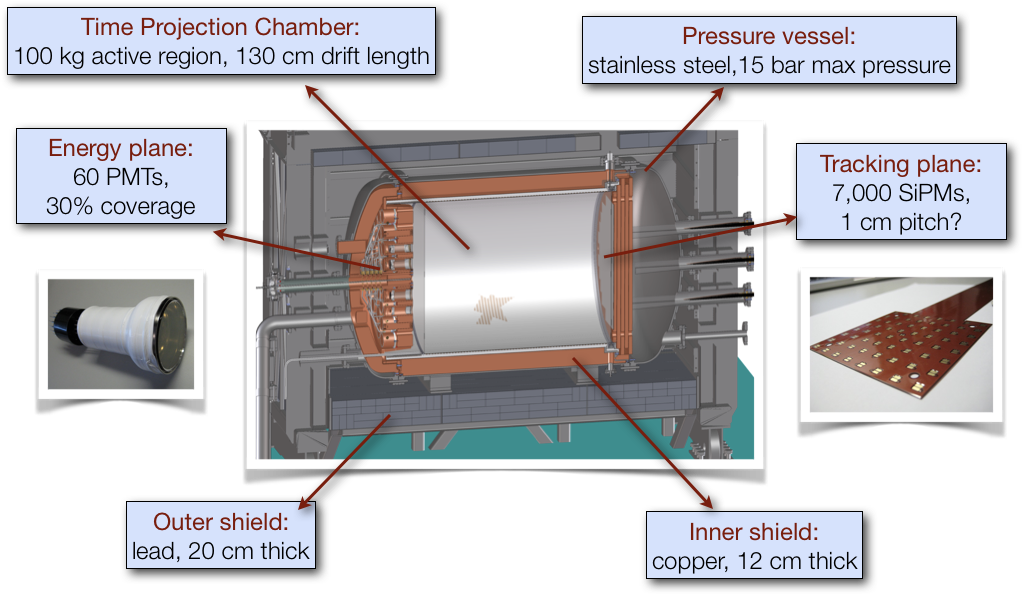
\includegraphics[width=0.75\textwidth]{moriond/next-100.png}   
  \end{center}
\end{figure}

\begin{itemize}
\item Scales up \NEW\ by roughly 2:1 in dimensions. 
\item Currently in construction. Commissioning in 2020. 
\end{itemize}
\end{frame}

\begin{frame}
\frametitle{Next-100 radioactive budget}
\begin{figure}[tbh!]
  \begin{center}
      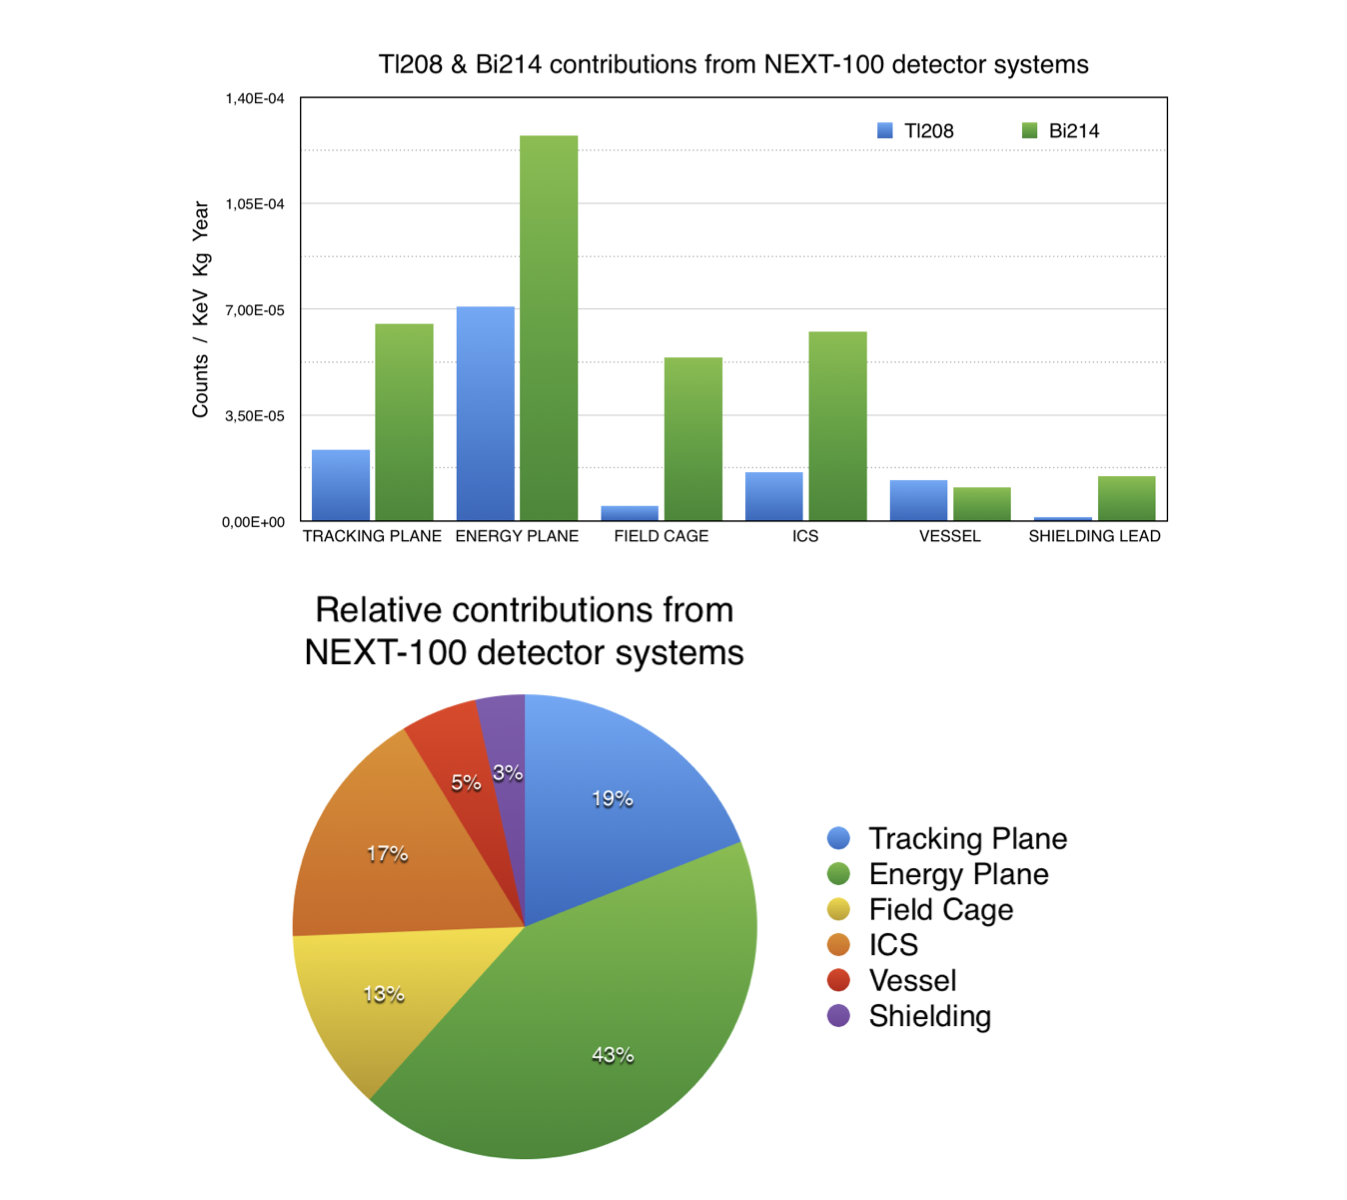
\includegraphics[width=0.6\textwidth]{moriond/next-100-radio_budget.png}
  \end{center}
 \end{figure}
 
\begin{itemize}
\item {\bf Expected background rate}, $ 4 \times 10^{-4} \ckky$. 
\item {\bf Expected background}, 1 event per year in ROI. 
\item {\bf Dominant source} PMTs. 
\end{itemize}
\end{frame}



 

\section{NEXT-2.0}
\begin{frame}
\frametitle{NEXT2-HD}

\begin{figure}[tbh!]
  \begin{center}
      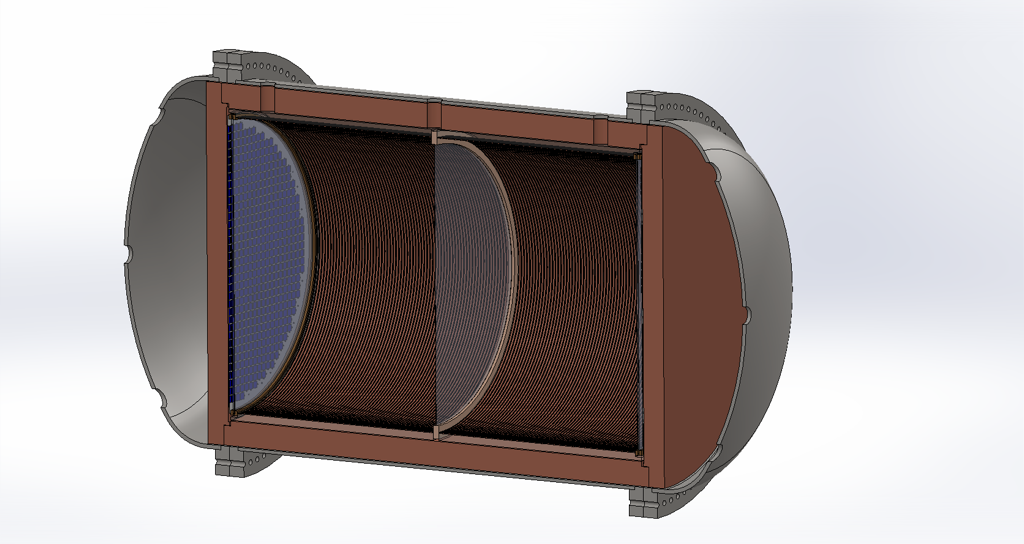
\includegraphics[width=0.75\textwidth]{moriond/next2.png}   
  \end{center}
\end{figure}

\begin{itemize}
\item Symmetric TPC: Diameter 2 m, drift length 3 m, pressure 20 bar, 1 ton per module.  
\item Uses only SiPMs mounted in ultra-pure substrates (gas cooled to -60 C).
  \item Low diffusion mixtures (Xe-He, Xe-CH$_4$). 
\end{itemize}
\end{frame}

\begin{frame}
\frametitle{NEXT2-HD improves rejection factor of topological signature}
\begin{figure}[tbh!]
  \begin{center}
      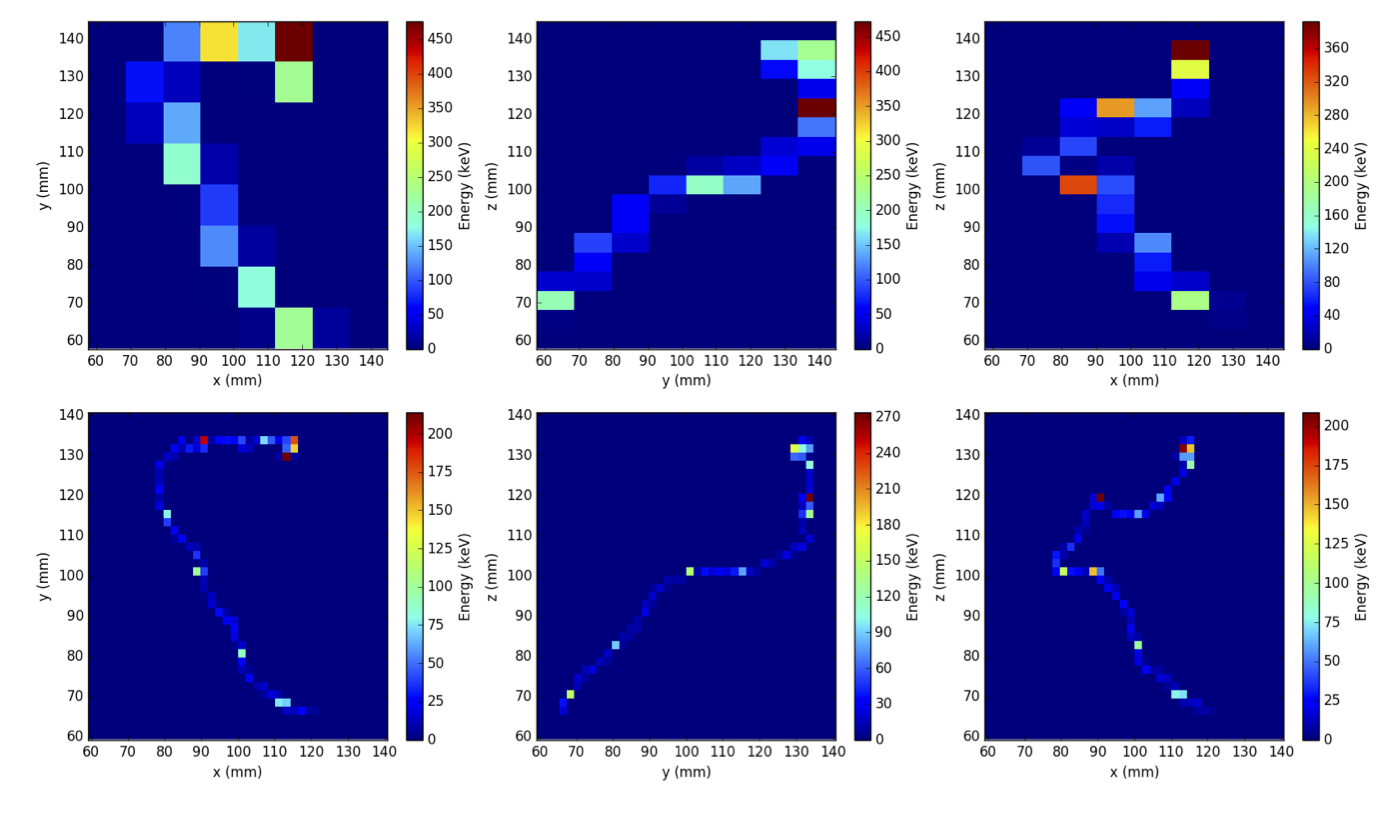
\includegraphics[width=0.45\textwidth]{moriond/high-low-diff-tracks.png}
       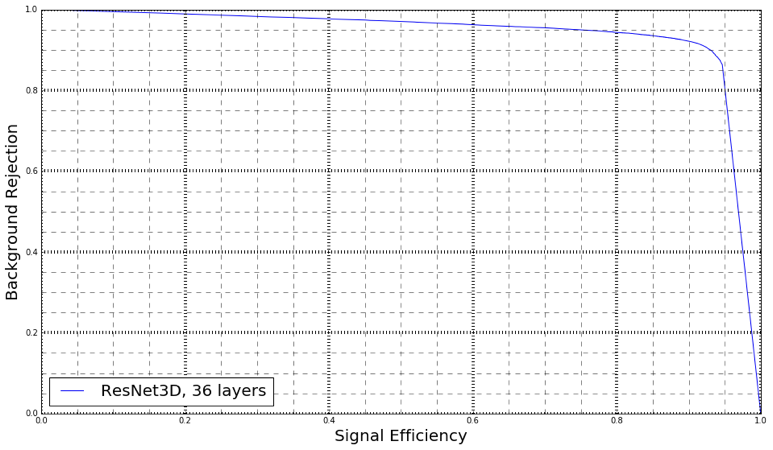
\includegraphics[width=0.45\textwidth]{moriond/signal-bkg-lowdiff-nn.png}
  \end{center}
 \end{figure}
 
 \begin{itemize}
\item Sharper topology results in an improvements of rejection factor by a factor 3.
\item Energy resolution may be further improved yielding a factor 2 (\BI\ peak very close to \Qbb).   
\end{itemize}
\end{frame} 

\begin{frame}
\frametitle{NEXT2-HD: incremental improvement approach}

\begin{columns}
 
\column{0.5\textwidth}
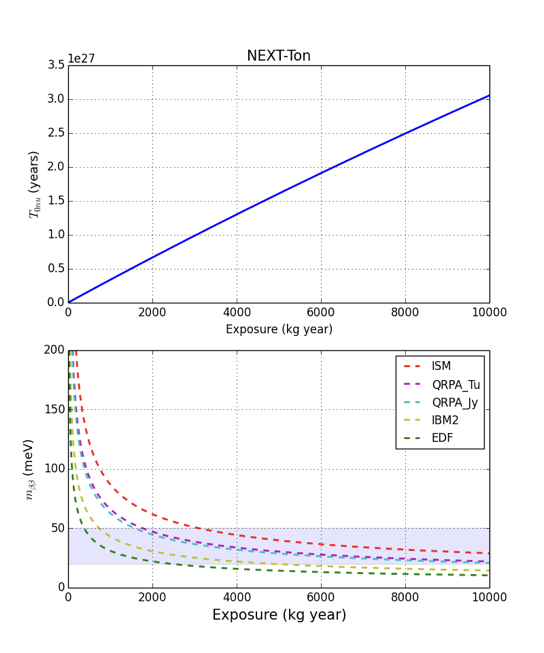
\includegraphics[scale=0.35]{moriond/next2-hd-sensi.png}
 
\column{0.5\textwidth}

%\begin{figure}[tbh!]
%  \begin{center}
%      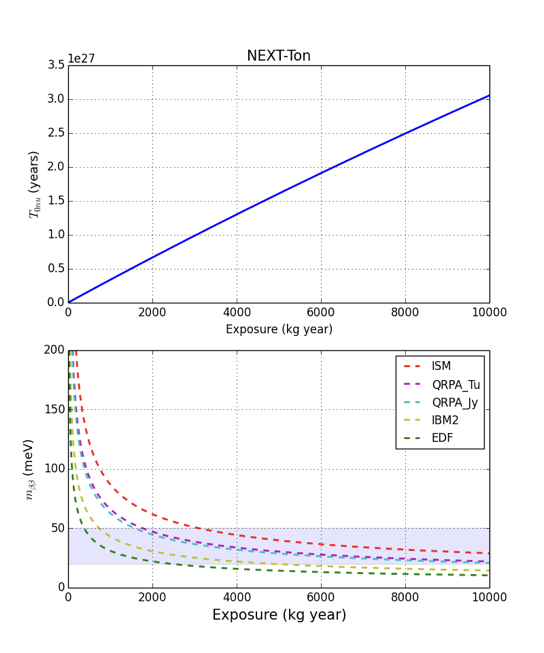
\includegraphics[width=0.4\textwidth]{moriond/next2-hd-sensi.png}
%   
%  \end{center}
% \end{figure}
 
\begin{itemize} 
\item SiPMs mounted in ultra-low background substrates, ultra-pure copper for inner shield, minimize materials inside TPC, deep underground location, water tank with neutron veto... an order of magnitude reduction in radioactive budget may be possible.   
\item Combination with improved topological signature and improved energy resolution may result in a ``background free'' detector at ton scale. 
\end{itemize}
\end{columns}
\end{frame}







 
\begin{frame}
\frametitle{NEXT2-BOLD}

\begin{figure}[tbh!]
  \begin{center}
      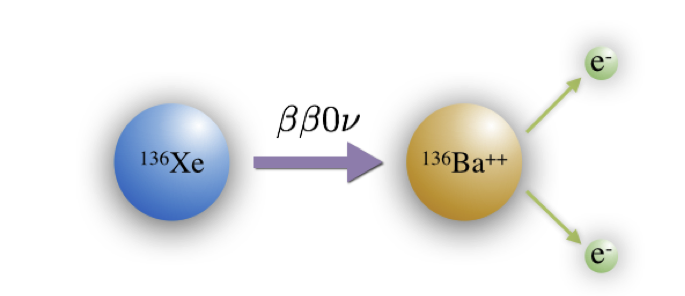
\includegraphics[width=0.75\textwidth]{moriond/bata.png}   
  \end{center}
\end{figure}
\begin{itemize} 
\item If the \Bapp\ produced in the $\XE \rightarrow \Bapp + 2 e (+ 2  \nu)$ can be detected efficiently, one could aim for the {\bf BOLD} (Barium iOn Light Detection) option.  
\item Detecting ``tagging'' the \Bapp\ signaling a \bbonu\ process has been a long sought holy grail of xenon chambers. 
\item Dave Nygren's proposal to do it using SMFI (Single Molecule Fluorescence Imaging) could turn fantasy into reality.   
\end{itemize}
\end{frame}

\begin{frame}
\frametitle{A bright idea}
  \begin{center}
      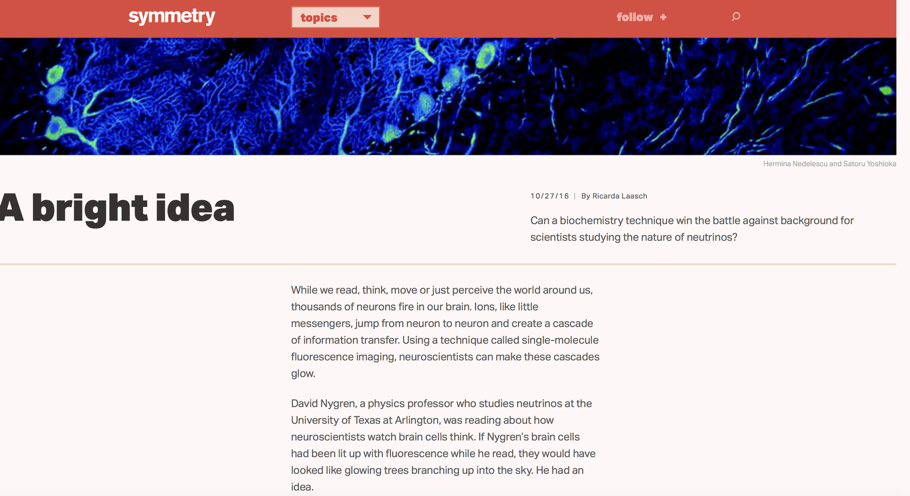
\includegraphics[width=0.75\textwidth]{moriond/nygren-smfi.png}   
  \end{center}
\begin{itemize} 
\item Dave Nygren's, 2016: \url{https://www.symmetrymagazine.org/article/a-bright-idea}    
\end{itemize}
\end{frame}

\begin{frame}
\frametitle{Single Molecule Fluorescence Imaging}
  \begin{center}
      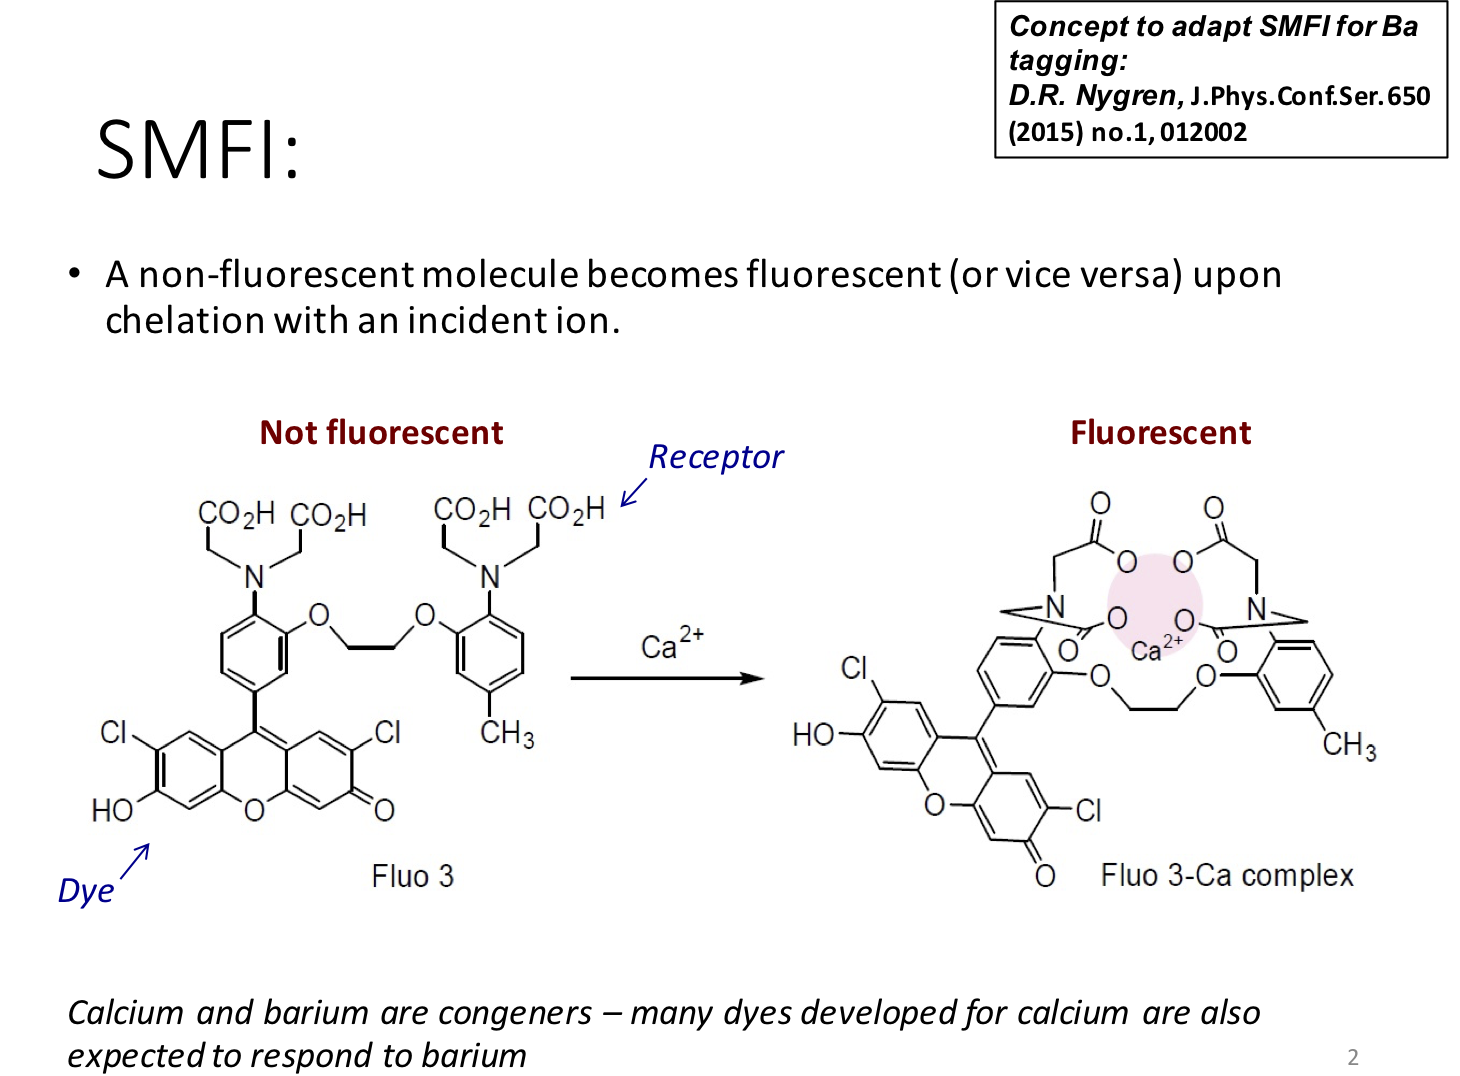
\includegraphics[width=0.75\textwidth]{moriond/smfi-concept.png}   
  \end{center}
\end{frame}

\begin{frame}
\frametitle{SMFI with \Bapp. Proof of concept}
  \begin{center}
      \includegraphics[width=0.85\textwidth]{moriond/sabat-poc.png}   
  \end{center}
\end{frame}

\begin{frame}
\frametitle{SMFI setup}
  \begin{center}
      \includegraphics[width=0.85\textwidth]{moriond/smfi-setup.png}   
  \end{center}
\end{frame}


\begin{frame}
\frametitle{We see single molecules chelated with \Bapp!}
  \begin{center}
      \includegraphics[width=0.85\textwidth]{moriond/smfi-observed.png}   
  \end{center}
\end{frame}



\begin{frame}
\frametitle{Next step? RITA}

\begin{columns}
 
\column{0.5\textwidth}
\includegraphics[scale=0.35]{moriond/rita.png}
 
\column{0.5\textwidth}

%\begin{figure}[tbh!]
%  \begin{center}
%      \includegraphics[width=0.4\textwidth]{moriond/next2-hd-sensi.png}
%   
%  \end{center}
% \end{figure}
 
\begin{itemize} 
\item RadIum TAgging (RITA) in dry medium (we can use several noble gases at different pressures).   
\item \Rapp\ produced by TH-228 decays. Radium and Barium are chemical "twin brothers" (same ionization potential, same radius, etc.). We can tag the production of \Rapp\ ions counting the recoiling alphas. 
\item Target will be a mon-layer of suitable molecules capable to capture the ion in gas and produce a strong fluorescence.
\item If RITA succeeds we may have a serious case for a BOLD NEXT-2.0 detector. 
\end{itemize}
\end{columns}
\end{frame}






 

\section{Summary and outlook}

\begin{frame}
\frametitle{Summary and outlook}
\begin{itemize} 
\item  After successful operation of the \NEW\ demonstrator we expect to commission NEXT-100 in 2020. 
\item We intend to operate NEXT-100 for about one year, to measure our background index and then upgrade the detector to a ``high-definition'' version, while we keep working in our SMFI barium tagging program. Thus we intend to keep open our option for an ``incremental" (HD) or ``disruptive'' (BOLD) NEXT-2.0 detector(s) aiming for exposures in the tens of ton year and extremely low backgrounds needed to maximize the chances of a discovery.   
\end{itemize}
\end{frame}
\begin{frame}

\frametitle{The NEXT collaboration}
  \begin{center}
      \includegraphics[width=0.85\textwidth]{moriond/next-coll.png}
  \end{center}
\end{frame}


\end{document}